%Movedopen
%\begin{wrapfigure}{r}{0.5\textwidth}
%	\vspace{-5mm}
%	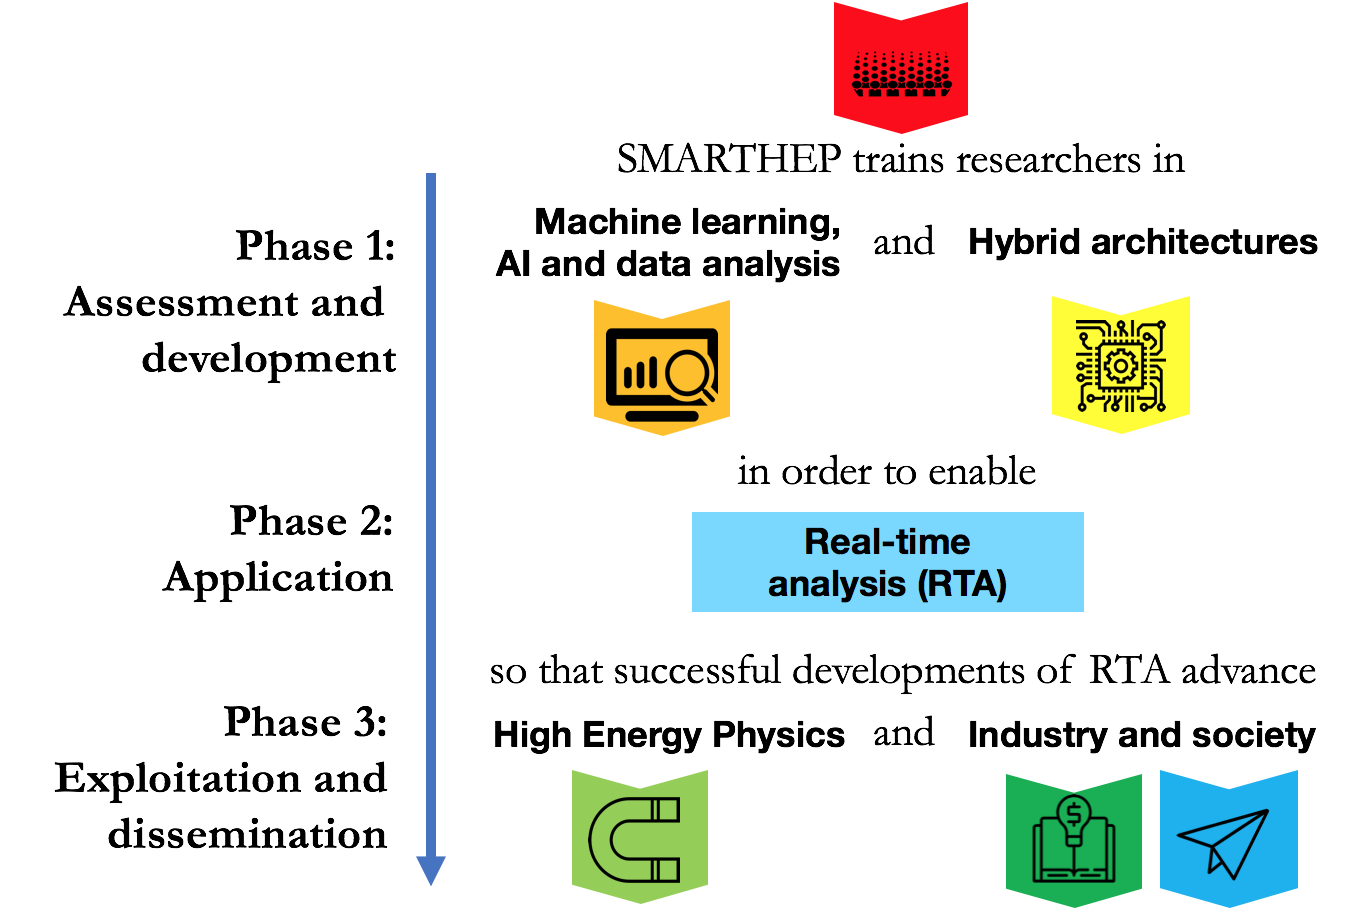
\includegraphics[width=0.49\textwidth]{figs/Implementation.png} %scienceStructure_2.pdf}
%    \vspace{-2mm} 
%	\caption{\acronym implementation strategy.\label{fig:implementation}}
%	\label{fig:scienceStructure.pdf}
%    \vspace{-10mm} 
%\end{wrapfigure}
%
%The connections between the different work packages and the overall \acronym strategy are shown in Fig.~\ref{fig:implementation}.
%Cutting-edge techniques in ML and hybrid architectures will be assessed and developed by the ESRs 
%before their application to specific use cases, in order to enable RTA that advance high energy physics, industry and society, 
%to follow with exploitation and dissemination as described in Sec.~\ref{sec:qualityExploitDissemination}. 
%This modus operandi is at the heart of \acronym and ensures the efficiency of its implementation. 

\subsubsection{Work Packages description}\label{sec:WPdescription}
\label{sub:WPsDescription}

%Earlier text
\acronym research topics and corresponding WPs have been introduced in Sec.~\ref{sec:metho}. 
The ESRs will work on projects which fall within different research WPs, strengthening \acronym into a coherent whole.
RTA is the conceptual and technical challenge which permeates all research work packages and motivates the network.
\vspace{-5mm}
%\newpage\clearpage
%Table 3.1.a

%WP1
%Description of Work and Role of Specific Beneficiaries / Partner Organisations
%(possibly broken down into tasks), indicating lead participant and role of other participants
\begin{center}\scriptsize
%\resizebox {\textwidth }{!}{%
\begin{tabular}{|p{0.05\textwidth}|p{0.15\textwidth}|p{0.23\textwidth}|p{0.15\textwidth}|p{0.12\textwidth}|}
\hline
\cellcolor{red!70!black} \textbf{\color{white}WP1\color{black}} & \textbf{Management} &  \textbf{Lead Beneficiary}: \lundentity & \textbf{Duration}: 1-48 & 
 ESR: 1 elected
\tabularnewline\hline
\multicolumn{5}{|p{0.975\textwidth}|}{%
\textbf{\Tstrut Objectives:} Create and  maintain a high level of collaboration between the \acronym consortium members to ensure the optimal functioning of the network, and report to the EU on network activities and progress.}\tabularnewline\hline
\multicolumn{5}{|p{0.975\textwidth}|}{\textbf{\Tstrut Description of Work and Role of Partners:}
Doglioni as Project Coordinator (PC) will oversee the smooth running of the planned research and training activities for the network.
\lund has been chosen to coordinate \acronym as a large institution with dedicated support and experience with projects of this kind, and due to Doglioni's experience in coordinating HEP communities and groups within and beyond ATLAS  (e.g. LHC Dark Matter Working Group, more than 300 participants and HEP Software Foundation trigger and reconstruction WG). 
Doglioni is an alumna of the \href{http://www.collegiocavalieri.it/en}{Collegio Universitario Lamaro Pozzani}, funded by the Italian National Federation of Holders of the Order of Merit for Labour and hosting up to 15 selected Italian students per year, complementing their regular university education with courses and lectures in entrepreneurship, law, IT and languages.
This gives her an unique perspective on cross-talk between academia and industry that started developing as early as her undergraduate education. 
Administrative support to the PC will be hired, at the level of at least 50\% FTE. %(\task{1.1}). 
The PC will keep close contact with other WP coordinators to monitor the execution of tasks, and  compliance to the defined milestones.
The PC's first task will be to convene discussions leading to the signature of the Consortium Agreement (CA). %(\task{1.2}).
Management will coordinate the hiring of all ESRs together with a dedicated recruitment officer.% (\task{1.3}, \task{1.4}).
The PC is responsible for preparing and chairing the consortium administrative meetings in the EB and SB, for the preparation of reports for the EU together with the project manager, and for overseeing the election of ESR representatives to the EB and SB. %(\task{1.5}), 
The PC and the relevant WP coordinators oversee the organization of the planned workshops and conferences % (\task{1.6}). 
The PC is responsible for facilitating communication between the nodes, building lasting collaborations between the nodes, enabling knowledge transfer and forming a legacy of future research collaborations.
\Bstrut}\tabularnewline\hline
\multicolumn{5}{|p{0.975\textwidth}|}{
	\pbox{202mm}{\textbf{\Tstrut Deliverables}: \deli{1.1} (month 2) Hiring of a dedicated project manager (month 1); \deli{1.2} Signature of the CA by all parties; }
	}\tabularnewline
\multicolumn{5}{|p{0.975\textwidth}|}{
\deli{1.3} (month 3) Launch of the website and social media accounts as outward-facing communication and organization tools;
}\tabularnewline
\multicolumn{5}{|p{0.975\textwidth}|}{
\deli{1.4} (month 3, 8) Advertisement of the recruitment and recruitment completion, including ESR declarations; 
}\tabularnewline
\multicolumn{5}{|p{0.975\textwidth}|}{
\deli{1.5}  (month 3, 13, 25, 37, 48)  Prepare reports for each SB meeting, incl. mandatory annual and mid-term progress report to EU ; 
}\tabularnewline
\multicolumn{5}{|p{0.975\textwidth}|}{
\deli{1.6}  (month 3, 13, 19, 25, 37, 43, 48)  Collect documentation, reports and feedback following all Network events and schools.
}%%	\pbox{202mm}{}
%%}
\tabularnewline\hline
\end{tabular}
%}%
%\vspace{-8mm}
\end{center}
%Table 3.1.a

%WP2
\begin{center}\scriptsize
\begin{tabular}{|p{0.05\textwidth}|p{0.15\textwidth}|p{0.23\textwidth}|p{0.15\textwidth}|p{0.12\textwidth}|}
\hline

\cellcolor{red} \textbf{\color{white}WP2\color{black}} & \textbf{Training} & \textbf{Lead Beneficiary}: \unige & \textbf{Duration: 1-48} & ESR: All\tabularnewline\hline

\multicolumn{5}{|p{0.975\textwidth}|}{%

\textbf{\Tstrut Objectives:} Organisation of the Network-wide training events, overview of the personal training for each ESR, see Sec.~\ref{sec:training}.}

\tabularnewline\hline
\multicolumn{5}{|p{0.975\textwidth}|}{\textbf{\Tstrut Description of Work and Role of Partners:}
The WP2 coordinator is Sfyrla from \unige, with experience in student supervision, public lectures and course organization. 
The WP2 coordinator oversees the preparation of the Personal Career Development Plans and follows up with the supervisors for the intermediate and final reports %(\task{2.1}). 
Prof. Sfyrla oversees the organization of the lectures for the development of technical, research and transferable skills (see Sec.~\ref{sec:trainingcontrib}) taking place at the Network-wide events. %(\task{2.2})..
The WP2 coordinator makes sure the lecturers give training of excellent quality and that adequate documentation is provided to the ESRs, and provides advertisement and follow-up material together with the PC.  
Short lecture proceedings will be prepared in advance of the lectures by the speakers so that they can be disseminated without delay following the events (as for example with the CHEP conference series). % (\task{2.3}), 
All nodes and partners will benefit and contribute to the training of the ESRs, by playing an active role through supervision of PhD programs, research and industry projects that will train excellent scientists with a wide range of skills and experiences. 
Together with the responsibles for WP7, Sfyrla will ensure the quality and feedback of the presentation of ESRs to \acronym events.% (\task{2.4})
\Bstrut}\tabularnewline\hline
\multicolumn{5}{|p{0.975\textwidth}|}{
	\pbox{202mm}{\textbf{\Tstrut Deliverables}: \deli{2.1}  (month 12, 24, 36, 42)  PCDPs for each ESR, intermediate and final monitoring;}
	}\tabularnewline
\multicolumn{5}{|p{0.975\textwidth}|}{
\deli{2.2}  (month 10, 15, 27-29, 38)  Design and organization of network-wide schools together with responsible beneficiaries;
}\tabularnewline
\multicolumn{5}{|p{0.975\textwidth}|}{
\deli{2.3}  (month 11, 16, 30, 39)  Proceedings of lectures given at the \acronym events; 
}\tabularnewline
\multicolumn{5}{|p{0.975\textwidth}|}{
\deli{2.4}  (month 12, 24, 36, 42)  Presentations from all ESR to the \acronym events and at the final conference;
}
\tabularnewline\hline
\multicolumn{5}{|p{0.975\textwidth}|}{
\deli{2.5} (month 44) ESRs with three-year PhD duration receive a degree.
}
\tabularnewline\hline
\end{tabular}
%\vspace{-9mm}
\end{center}

%%WP3
\begin{center}\scriptsize
\begin{tabular}{|p{0.04\textwidth}|p{0.24\textwidth}|p{0.21\textwidth}|p{0.12\textwidth}|p{0.07\textwidth}|}
\hline

\cellcolor{orange} \textbf{\color{black}WP3\color{black}} & \textbf{ML \& advanced data analysis} & \textbf{Lead Beneficiary}: \cnrs & \textbf{Duration: 8-48} & ESR: All \tabularnewline\hline

\multicolumn{5}{|p{0.975\textwidth}|}{%

\textbf{\Tstrut Objectives:} Deployment of advanced Machine Learning (ML) and data analysis techniques to enable real-time analysis.}

\tabularnewline\hline
\multicolumn{5}{|p{0.975\textwidth}|}{\textbf{\Tstrut Description of Work and Role of Partners:}
The WP3 coordinator is Gligorov from \cnrs, who led the first large-scale implementation of real-time ML at an LHC experiment in 2011, led LHCb's HLT during 2014 and 2015, oversaw LHCb's physics programme as deputy physics coordinator during 2016 and 2017 and is currently leader of the Real Time Analysis Project in LHCb.  
The WP3 coordinator is responsible for the coherence and interaction of the ESRs investigating ML techniques in RTA throughout \acronym, for their development and their application to HEP and commercial use cases according to the network-wide strategy described in Fig.~\ref{fig:implementation}. 
He will also ensure that code is written alongside documentation that makes the software useful and usable, and that frameworks and toolkits are made public in a timely manner and respecting IP clauses in case of commercial exploitation. 
WP3 will produce novel algorithms to reconstruct objects and events in real-time (with the know-how of \nikhefentity and \cernentity), and develop ML techniques for event reconstruction, fast data analysis and outlier detection (exploiting the expertise of \liegesentity, \ibmentity, \fleetmaticsentity and \unigeentity). 
The algorithms for both reconstruction and ML will also be benchmarked and optimized in the projects hosted at \nikhefentity and \cernentity. 
\Bstrut}\tabularnewline\hline
\multicolumn{5}{|p{0.975\textwidth}|}{
\textbf{\Tstrut Deliverables}: \textit{For this and other research WP deliverables, we follow the implementation plan in ~\ref{sec:introRO}, where the ESRs first gain an overview of the state of the art, then developing new techniques, and finally disseminating them as legacy of \acronym.}} 
\tabularnewline
\multicolumn{5}{|p{0.975\textwidth}|}{
\deli{2.2} (joint with WP1, WP2) design, organization and documentation of the contributions to the network ML and MLHEP schools
}\tabularnewline
\multicolumn{5}{|p{0.975\textwidth}|}{
\deli{\deliverableWhitepaperStateOfTheArtWPThree}  (month \deliverableWhitepaperStateOfTheArtWPThreeMonth) 
Whitepaper on the state of the art on ML for real-time analysis, detailing implementation and deployment, capitalizing on the attendance of the MLHEP school in month  24;
}\tabularnewline
\multicolumn{5}{|p{0.975\textwidth}|}{
\deli{\deliverableTriggerExperimentalSoftwareWPThree}  (month \deliverableTriggerExperimentalSoftwareWPThreeMonth) 
Collection of ML algorithms and software toolkits to be exploited for the research objectives in WP5 and WP6; 
}\tabularnewline
\multicolumn{5}{|p{0.975\textwidth}|}{
\deli{\deliverableFinalWhitepaperWPThree}  (month \deliverableFinalWhitepaperWPThreeMonth) .
Review paper collecting description and documentation of techniques for ML in RTA. 
}
\tabularnewline\hline
\end{tabular}
%\vspace{-9mm}
\end{center}


%%WP4
\begin{center}\scriptsize
\begin{tabular}{|p{0.04\textwidth}|p{0.18\textwidth}|p{0.17\textwidth}|p{0.12\textwidth}|p{0.20\textwidth}|}
\hline

\cellcolor{yellow} \textbf{\color{black}WP4\color{black}}  & \textbf{Hybrid architectures} & \textbf{Lead Beneficiary}: \sorbonneentity & \textbf{Duration: 8-48}  & ESR: \ESRsForWPFourText \tabularnewline\hline

\multicolumn{5}{|p{0.975\textwidth}|}{%

\textbf{\Tstrut Objectives:} Study and adoption of hybrid computing architectures to enable RTA.}

\tabularnewline\hline
\multicolumn{5}{|p{0.975\textwidth}|}{\textbf{\Tstrut Description of Work and Role of Partners:}
The WP4 coordinator is Lacassagne from \sorbonneentity. 
He is a system architect with extensive experience in the benchmarking and use of hybrid architectures. 
The WP4 coordinator is responsible for the coherence and interaction of the ESRs developing and testing code for hybrid architectures. 
He is responsible for the  publication and exploitation of successful deliverables related to hybrid architectures, as well as many studies that demonstrated that standard architectures could be improved for the purpose of RTA (see e.g. Lemaitre, Lacassagne, \href{https://hal.archives-ouvertes.fr/hal-01361204/document}{Batched Cholesky Factorization for tiny matrices}, DASIP 2016).
The work is divided in three tasks corresponding to the research objectives: the use of FPGAs (e.g. track triggering for ATLAS, expertise of \ohioentity, \oregonentity, \pisaentity), the use of GPUs for speeding up parallel algorithms in industry and HEP (\santiagoentity), and employing parallel and multithreaded algorithms (\lightboxentity).
Together with the partners, the WP4 coordinator also oversees the training program on each specific architecture, and ensures the quality of lectures and their proceedings with the coordinator of WP2. 
He also makes sure that code written for non-standard architectures satisfies high documentation standards.
\Bstrut}\tabularnewline\hline
\multicolumn{5}{|p{0.975\textwidth}|}{
\textbf{\Tstrut Deliverables}: \deli{2.2} (joint with WP1, WP2) design, organization and documentation of the FPGA and GPU schools.} 
\tabularnewline
\multicolumn{5}{|p{0.975\textwidth}|}{
\deli{\deliverableWhitepaperStateOfTheArtWPFour}  (month \deliverableWhitepaperStateOfTheArtWPFourMonth)  
Whitepaper on the state of the art on hybrid architectures in real-time analysis, capitalizing on attendance of network FPGA/GPU schools;
}\tabularnewline
\multicolumn{5}{|p{0.975\textwidth}|}{
\deli{\deliverableParallelizationOptimizationWPFour}  (month \deliverableParallelizationOptimizationWPFourMonth) 
Software toolkits and hardware improvements in HEP (e.g. FTK for ATLAS, GPU for LHCb reconstruction); 
}\tabularnewline
\multicolumn{5}{|p{0.975\textwidth}|}{
\deli{\deliverableParallelization}  (month \deliverableParallelizationMonth) 
\lightbox software to optimize parallelization of financial transactions and associated publications; 
}\tabularnewline
\multicolumn{5}{|p{0.975\textwidth}|}{
\deli{\deliverableWhitepaperDevelopmentWPFour}  (month \deliverableWhitepaperDevelopmentWPFourMonth)  
Review paper collecting advancements in optimization of hybrid architectures for the LHC trigger systems.
}
\tabularnewline\hline
\end{tabular}
%\vspace{-9mm}
\end{center}

%%WP5
\begin{center}\scriptsize
\begin{tabular}{|p{0.04\textwidth}|p{0.23\textwidth}|p{0.20\textwidth}|p{0.12\textwidth}|p{0.12\textwidth}|}
\hline

\cellcolor{green} \textbf{\color{black}WP5\color{black}} & \textbf{Real-time decision making} & \textbf{Lead Beneficiary}: \dortmundentity & \textbf{Duration: 8-48} 
&   ESR: \ESRsForWPFiveText \tabularnewline\hline

\multicolumn{5}{|p{0.975\textwidth}|}{%

\textbf{\Tstrut Objectives:}  Applying real-time analysis to decision making in physics and society.}

\tabularnewline\hline
\multicolumn{5}{|p{0.975\textwidth}|}{\textbf{\Tstrut Description of Work and Role of Partners:}
WP5's goal is to enable fast and efficient decision making with RTA, in physics through the use of the trigger systems, and in society to improve safety and efficiency of transport in ways that would not be possible without RTA. 
WP5 is coordinated by Albrecht (\dortmundentity as main beneficiary node) with Sopasakis as co-coordinator (\ximantis). 
They have been chosen to fill this role for their complementary expertise in decision-making in HEP and industry that are crucial for \acronym. 
%trigger strategies crucial for the physics analyses in \acronym, and for their expertise on RTA decision-making in transport. 
They will ensure that the RTA techniques enabled by WP3 and WP4 are applied to advance both HEP and industry by the various ESRs working on the experiment trigger systems, that the exchange between academia and industry is fruitful in both directions through cross-pollination of techniques, and that the results are documented in peer-reviewed papers. 
%Together with the WP2 and WP3 coordinators, they oversee the trigger lectures in the introductory event at \lund and the physics and ML school at \unigeshort, and coordinate the preparation of the ISOTDAQ and MLHEP lectures and ESR contributions.
\Bstrut}\tabularnewline\hline
\multicolumn{5}{|p{0.975\textwidth}|}{
\textbf{\Tstrut Deliverables}: \deli{2.2} (joint with WP1, WP2) organization of trigger contributions to network events and ISOTDAQ schools.} 
\tabularnewline
\multicolumn{5}{|p{0.975\textwidth}|}{
\deli{\deliverableWhitepaperStateOfTheArtWPFive}  (month \deliverableWhitepaperStateOfTheArtWPFiveMonth) 
Review of the state of the art of the triggers of LHC collaborations, compiled by ESRs will prior to their physics analyses capitalizing on attendance of ISOTDAQ school and network events; 
}\tabularnewline
\multicolumn{5}{|p{0.975\textwidth}|}{
\deli{\deliverableXimantisHybrid}  (month \deliverableXimantisHybridMonth) 
Improved \ximantisentity app using novel ML techniques (e.g. hybrid networks) and associated publications;
}\tabularnewline
\multicolumn{5}{|p{0.975\textwidth}|}{
\deli{\deliverableTriggerExperimentalSoftwareWPFive}  (month \deliverableTriggerExperimentalSoftwareWPFiveMonth) 
Software for LHC trigger upgrades for Run-3 data taking; 
}\tabularnewline
\multicolumn{5}{|p{0.975\textwidth}|}{
\deli{\deliverableLogisticsOptimisation}  (month \deliverableLogisticsOptimisationMonth) 
Client software for optimization of transport and logistics with \pointeightentity and associated publications;
}
\tabularnewline
\multicolumn{5}{|p{0.975\textwidth}|}{
\deli{\deliverableWhitepaperCollectionPapersWPFive}  (month \deliverableWhitepaperCollectionPapersWPFiveMonth)  
Review paper collecting physics results using trigger selection improvements, including summary of publications on dark sectors, LFV/LFU and precision measurements.}
\tabularnewline\hline

\end{tabular}
%\vspace{-9mm}
\end{center}

%%WP6
\begin{center}\scriptsize
\begin{tabular}{|p{0.04\textwidth}|p{0.3\textwidth}|p{0.18\textwidth}|p{0.12\textwidth}|p{0.2\textwidth}|}
\hline

\cellcolor{cyan} \textbf{\color{black}WP6\color{black}} & \textbf{Real-time monitoring and discoveries} & \textbf{Lead Beneficiary}: \ibm & \textbf{Duration: 8-48} &
ESR: \ESRsForWPSixText \tabularnewline\hline

\multicolumn{5}{|p{0.975\textwidth}|}{%

\textbf{\Tstrut Objectives:}   Applying real-time analysis to monitor complex systems and discover anomalies, in physics and society.}

\tabularnewline\hline
\multicolumn{5}{|p{0.975\textwidth}|}{\textbf{\Tstrut Description of Work and Role of Partners:}
The goal of WP6 is to employ real-time analysis to detect novelty or anomalies while monitoring complex systems and streams of data. 
These data streams range from LHC collision events (\lundentity), to financial transactions (\ibmentity), to data from vehicle dashboard cameras (\fleetmaticsentity), to sensor data from industrial processes (\lightboxentity). 
A sub-goal that is novel to \acronym and essential to introduce such techniques in HEP trigger systems is the accountability and reproducibility of the algorithms employed, developed in \ESRx. 
For this reason, \ibmentity is chosen as the lead beneficiary of WP6 with De Sainte Marie as main coordinator, given his extensive experience in supervision of student projects and his expertise on symbolic knowledge systems. 
WP6's academic co-coordinator is Pierini (\cern), one of the pioneers of anomaly detection in LHC experiments. 
WP6 will work in close collaboration with WP3 to design new algorithms and combine the best of both symbolic knowledge and numerical algorithms towards application to HEP triggers and society. 
The deliverables of WP6 match the research objectives and include applications both in HEP and in the commercial sector, as the algorithms developed can be ported to the different kinds of data. 
Aided by the WP7 coordinator, by LU Innovation from the PC side and by the H2020 IPR helpdesk, WP6 coordinators ensure that these commercial deliverables are disseminated and documented after their exploitation, and correctly handled in terms of IP and \href{http://ec.europa.eu/justice/data-protection/index_en.htm}{EU GDPR}.
\Bstrut}\tabularnewline\hline
\multicolumn{5}{|p{0.975\textwidth}|}{
\textbf{\Tstrut Deliverables}: \deli{2.2} (joint with WP1, WP2) organization of the non-academic training and Industry and career development schools. } 
\tabularnewline
\multicolumn{5}{|p{0.975\textwidth}|}{
\deli{\deliverableWhitepaperStateOfTheArtWPSix} 
Review of the state of the art of fully RTA searches in HEP and recommendations for improvements (companion of \deli{\deliverableWhitepaperStateOfTheArtWPFive})
 (month \deliverableWhitepaperStateOfTheArtWPSixMonth) ; 
}\tabularnewline

\multicolumn{5}{|p{0.975\textwidth}|}{
\deli{\deliverableSoftwareWPSix}  (month \deliverableSoftwareWPSixMonth) 
Software enabling advanced fully RTA-based searches at LHC; 
}\tabularnewline

\multicolumn{5}{|p{0.975\textwidth}|}{
\deli{\deliverableRule}  (month ~\deliverableRuleMonth) 
Algorithms for fraud detection and HEP triggers in \ibmentity and associated publications;
}\tabularnewline

\multicolumn{5}{|p{0.975\textwidth}|}{
\deli{\deliverableFleetmaticsMLMobile}  (month \deliverableFleetmaticsMLMobileMonth) 
Toolkits using ML and AI for real-time in-fleet monitoring within \fleetmaticsentity and associated publications;
}

\tabularnewline
\multicolumn{5}{|p{0.975\textwidth}|}{
\deli{\deliverablePredictiveMaintenance}  (month \deliverablePredictiveMaintenanceMonth) 
Software for sensors for Internet-of-things and industrial process optimization in \lightboxentity 
}
\tabularnewline
\multicolumn{5}{|p{0.975\textwidth}|}{
\deli{\deliverableWhitepaperCollectionPapersWPSix}  (month \deliverableWhitepaperCollectionPapersWPSixMonth)  
Review paper collecting physics results using fully RTA-based analyses, including summary of publications on dark matter mediators, Higgs boson, heavy ion physics. 
%%Companion paper on summary of technical work, and implications outside HEP. 
}
\tabularnewline\hline
\end{tabular}
%\vspace{-9mm}
\end{center}

%%WP7
\begin{center}\scriptsize
\begin{tabular}{|p{0.04\textwidth}|p{0.23\textwidth}|p{0.20\textwidth}|p{0.12\textwidth}|p{0.12\textwidth}|}
\hline

\cellcolor{violet} \textbf{\color{black}WP7\color{black}} & \textbf{Outreach and dissemination} & \textbf{Lead Beneficiary}: \cern & \textbf{Duration: 1-48} & ESR: All ESRs.\tabularnewline\hline

\multicolumn{5}{|p{0.975\textwidth}|}{%


\textbf{\Tstrut Objectives:} Relay \acronym scientific activities to the general public, monitor delivery of results as journal papers, ensure ESR visibility in conferences.}
\tabularnewline\hline

\multicolumn{5}{|p{0.975\textwidth}|}{\textbf{\Tstrut Description of Work and Role of Partners:}
WP7 is detailed further in Sec.~\ref{sec:CommPub}.  
\cern is chosen as the lead beneficiary of WP7 given its extensive experience in communicating with the public, with Petersen as responsible. 
Ustyuzhanin from \yandexentity will co-coordinate the effort benefitting from his extensive expertise with data challenges. 
The WP7 coordinator organise the communication of \acronym to both the general public and the scientific community and ensure that all ESRs and supervisors take part in the effort. 
Together with the PC they run the dedicated communication portal \url{www.smarthep.org}, supported by ESR blogging and social media activities. 
Communication to the scientific communities is achieved by poster and talk contributions to conferences. 
The WP7 coordinator will delegate members of the network to support the ESR supervisors and monitor the quality of the material presented by the ESRs and ensure they benefit from an outstanding international visibility. 
The coordinators will ensure a consistent top quality of papers produced within the Network. 
The main innovation of \acronym's outreach program is the ESR data challenge, organized by \cernentity. 
Further outreach to the general public will take the form of visits to schools, guided visits to CERN facilities, public lectures and "science on tap" at Network events. 
\acronym dissemination activities will be completed by delivery of the specific \acronym Masterclass exercise.
These tasks will ensure the general public grasps the impact of \acronym on academia and HEP, industry and everyday life and actively participates in it through the data challenge.
All academic and industrial partners will take an active part in the WP7 activities, and will simultaneously host online the International Masterclass exercises and World Wide Data Day (WWDD) activities, including on the International Day of Women in Science day.
}\tabularnewline\hline
\multicolumn{5}{|p{0.975\textwidth}|}{
\textbf{\Tstrut Deliverables}: 
\deli{1.3}  (joint with WP1)  Launch of \url{www.smarthep.org} and social media as platform for dissemination, communication and outreach;
}\tabularnewline
\multicolumn{5}{|p{0.975\textwidth}|}{
\deli{7.1}  (month 14)  Data challenge website online and open to the public; 
}\tabularnewline
\multicolumn{5}{|p{0.975\textwidth}|}{
\deli{7.2}  (month 24, 36, 48)  Report on presentation of results at international conferences; 
}\tabularnewline
\multicolumn{5}{|p{0.975\textwidth}|}{
\deli{7.3}  (month 24, 36, 48)  Report on publication of results in peer-reviewed journals; 
}\tabularnewline
\multicolumn{5}{|p{0.975\textwidth}|}{
\deli{7.4}  (month 12, 24, 36, 48)  Reports on outreach to the general public and on \acronym Masterclass/WWDD exercise.
}

\tabularnewline\hline
\multicolumn{5}{p{0.975\textwidth}}{\textbf{Table 3.1a} Work package description for each work package.}
\end{tabular}
%%\vspace{-9mm}
\end{center}

\FloatBarrier
%\clearpage

\subsubsection{List of major deliverables}
\label{sub:deliverables}

%A deliverable is a distinct output of the action, meaningful in terms of the action?s overall objectives and constituted by a report, a document, a technical diagram, a software, training, conference, etc. These should be divided into scientific deliverables and management, training, recruitment and dissemination deliverables. Scientific deliverables have technical/scientific content specific to the action. The number of deliverables in a given Work Package must be reasonable and commensurate with the Work Package content. Note that during implementation, the submission of these deliverables to the REA will be a contractual obligation.
%Table 3.1.b, Including the awarding of doctoral degrees!
%\vspace{-1mm}
The following tables list the deliverables of the project. 

\color{blue}\noindent Scientific Deliverables\color{black}\addtocounter{table}{1} \vspace{-9mm}\\
\begin{center}
\scriptsize
%\resizebox {\textwidth }{!}{%
\begin{tabular}{@{}p{5mm}@{~~}p{105mm}p{6mm}p{18mm}p{6mm}cp{8mm}@{}}
\toprule
\multicolumn{2}{l}{\pbox{8cm}{Deliverable Number \& Title}} &
%Deliverable numbers in order of delivery dates. Please use the numbering convention <WP number>.<number of deliverable within that WP>. For example, deliverable 4.2 would be the second deliverable from Work Package 4.
WP &
\pbox{8cm}{\Tstrut Lead Benef.\\Short Name\Bstrut}& %\\Short\\Name
\multicolumn{2}{c}{\pbox{8cm}{Type \& Dissemin.\\Level}}&
%Type: Please indicate the nature of the deliverable using one of the following codes:
%R = Report; ADM = Administrative (website completion, recruitment completion, etc.); 
%PDE = dissemination and/or exploitation of results; OTHER = Other, including coordination 

%Dissemination level:
%Please indicate the dissemination level using one of the following codes:	
%PU = Public: fully open, e.g. web; 
%CO = Confidential: restricted to consortium, other designated entities (as appropriate) and Commission services; 
%Please consider that deliverables marked as "PU" will automatically be published on CORDIS once approved: the applicants should 
%therefore consider the relevance of marking a deliverable as "PU";
%CI = Classified: classified information as intended in Commission Decision 2001/844/EC. 
\pbox{8cm}{Due\\Date} 
%Description
\tabularnewline 
\toprule

%20
\deli{\deliverableWhitepaperStateOfTheArtWPFive} & 
Review of the state of the art of the triggers of LHC collaborations and best practices&
5 & \dortmundentity & R & PU & \deliverableWhitepaperStateOfTheArtWPFiveMonth 
%20
\tabularnewline\midrule 
\deli{\deliverableWhitepaperStateOfTheArtWPSix} & 
Whitepaper on the state of the art of fully RTA-based searches in HEP and best practices&
6 & \ibmentity & R & PU & \deliverableWhitepaperStateOfTheArtWPSixMonth 
%24
\tabularnewline\midrule 
\deli{\deliverableWhitepaperStateOfTheArtWPThree} & 
Whitepaper summarizing the state of the art in ML techniques for RTA and best practices& 
3 & \cnrs & R & PU & \deliverableWhitepaperStateOfTheArtWPThreeMonth 
%29
\tabularnewline\midrule 
\deli{\deliverableLogisticsOptimisation} & 
Client software for optimization of transport with \pointeightentity and associated publications &
5 & \dortmundentity & OTHER & CO & \deliverableLogisticsOptimisationMonth
%29
\tabularnewline\midrule 
\deli{\deliverableWhitepaperStateOfTheArtWPFour} & 
Whitepaper on the state of the art on hybrid architectures in real-time analysis &
4 & \sorbonneentity & R & PU & \deliverableWhitepaperStateOfTheArtWPFourMonth
%31
\tabularnewline\midrule 
\deli{\deliverablePredictiveMaintenance} &
Software for sensors for Internet-of-things and industrial process optimization in \lightboxentity &
6 & \ibmentity & OTHER & CO & \deliverablePredictiveMaintenanceMonth
%32
\tabularnewline\midrule 
\deli{\deliverableTriggerExperimentalSoftwareWPThree} & 
ML algorithms and software enabling RTA at LHC during Run-2 data taking  & 
3 & \cnrs & OTHER & CO & \deliverableTriggerExperimentalSoftwareWPThreeMonth
%32
\tabularnewline\midrule 
\deli{\deliverableTriggerExperimentalSoftwareWPFive} &
Software for LHC trigger upgrades for Run-3 data taking &
5 & \dortmundentity & OTHER & CO & \deliverableTriggerExperimentalSoftwareWPFiveMonth
%32
\tabularnewline\midrule 
\deli{\deliverableSoftwareWPSix} & 
Software enabling advanced fully RTA-based searches at LHC &
6 & \ibmentity & OTHER & CO & \deliverableSoftwareWPSixMonth 
%35
\tabularnewline\midrule 
\deli{\deliverableFinalWhitepaperWPThree} & 
Review paper collecting ML and data analysis advancements from ESR projects & 
3 & \cnrs & PDE & PU & \deliverableFinalWhitepaperWPThreeMonth 
%35
\tabularnewline\midrule 
\deli{\deliverableParallelization} & 
\lightboxentity software to optimize parallelization of financial transactions, associated publications &
4 & \cnrs & OTHER & CO & \deliverableParallelizationMonth 
%36
\tabularnewline\midrule 
\deli{\deliverableXimantisHybrid} & 
Improved \ximantisentity app (e.g. using hybrid/Attention ML networks) and associated publications &
5 & \dortmundentity & OTHER & CO & \deliverableXimantisHybridMonth 
%39
\tabularnewline\midrule 
\deli{\deliverableParallelizationOptimizationWPFour} & 
Software toolkits and hardware improvements in HEP (e.g. FTK for ATLAS, GPU for LHCb) &
4 & \cnrs & OTHER & CO & \deliverableParallelizationOptimizationWPFourMonth
%40
\tabularnewline\midrule 
\deli{\deliverableFleetmaticsMLMobile} & 
Toolkits for real-time fleet monitoring within \fleetmaticsentity and associated publications &
6 & \ibmentity & OTHER & CO & \deliverableFleetmaticsMLMobileMonth
%40
\tabularnewline\midrule 
\deli{\deliverableRule} & 
Algorithms for fraud detection and HEP triggers in \ibmentity and associated publications &
6 & \ibmentity & OTHER & CO & \deliverableRuleMonth
%42
\tabularnewline\midrule 
\deli{\deliverableWhitepaperDevelopmentWPFour} &
Review paper collecting advancements in optimization of hybrid architectures for LHC triggers &
4 & \cnrs & PDE & PU & \deliverableWhitepaperDevelopmentWPFourMonth
%42
\tabularnewline\midrule 
\deli{\deliverableWhitepaperCollectionPapersWPSix} & 
Review paper collecting ESR physics results using fully RTA-based analyses &
6 & \ibmentity & PDE & PU & \deliverableWhitepaperCollectionPapersWPSixMonth 
%42
\tabularnewline\midrule 
\deli{\deliverableWhitepaperCollectionPapersWPFive} & 
Review paper collecting ESR physics results using trigger selection improvements &
5 & \dortmundentity & PDE & PU & \deliverableWhitepaperCollectionPapersWPFiveMonth 

\label{tab:DeliverList}
\end{tabular}
%}%
%\vspace{-8mm}
\end{center}
%\noindent Scientific Deliverables (contd) \addtocounter{table}{1}\vspace{-6mm}\\

\noindent \color{blue} Management, Training, Recruitment and Dissemination Deliverables\color{black}\addtocounter{table}{1}\vspace{-5mm}\\
% 	Including overall recruitment (e.g. advertising vacancies), Researcher Declarations on Conformity, Career development Plan, training deliverable x, etc. The individual recruitments should only be listed in Table 1.2a 
\begin{center}
\scriptsize
%\resizebox {\textwidth }{!}{%
\begin{tabular}{@{}p{5mm}@{~~}p{100mm}p{6mm}p{10mm}p{6mm}cp{20mm}@{}}
%\begin{tabular}{@{}p{5mm}@{~~}p{95mm}p{4mm}p{10mm}p{6mm}cp{12mm}@{}}
\toprule
\multicolumn{2}{l}{\pbox{8cm}{Deliverable Number \& Title}} &
WP &
\pbox{8cm}{\Tstrut Lead Benef.\\Short Name\Bstrut}&
\multicolumn{2}{c}{\pbox{8cm}{Type \& Dissemin.\\Level}}&
\pbox{8cm}{Due\\Date} 
\tabularnewline 
\toprule
\deli{1.1} & Project manager hired  at the PC's institute & 1 & \lundentity & ADM & CO & 2 \tabularnewline\midrule
\deli{1.2} & Signature of Consortium Agreement by all parties & 1 & \lundentity & ADM & CO & 2 \tabularnewline\midrule
\deli{1.3} & Launch of the website and social media accounts & 1,7 & \lundentity & PDE & PU & 3  \tabularnewline\midrule
\deli{1.4} & Advertisement, selection and recruitment of all ESRs & 1 & \lundentity & ADM & CO & 3, 8  \tabularnewline\midrule
\deli{1.5} & EB/SB meeting minutes and EU reports  & 1 & \lundentity & R & CO & 3,13,25,37,48  \tabularnewline\midrule
\deli{1.6} & Collect documentation, reports and feedback for all Network events and schools. & 1 & \lundentity & R & PU/PDE & 3,13,19,25,37,48 \tabularnewline\midrule
\deli{2.2} & Design and organization of network-wide schools together with other responsibles & 2-6 & \unigeentity & OTHER & CO & 10, 15, 27-29, 38 \tabularnewline\midrule
\deli{2.1} & Preparation, network approval and monitoring of PCDP & 2 & \unigeentity & OTHER & CO & 12, 24, 36, 42 \tabularnewline\midrule
\deli{7.4} & Reports on commmunication, outreach and \acronym Masterclass/WWDD. & 7 & \cernentity & R & PU & 12, 24, 36, 48 \tabularnewline\midrule
\deli{2.3} & Publication of \acronym school \& event proceedings on website & 2 & \unigeentity & PDE & PU & 11, 16, 30, 39 \tabularnewline\midrule
\deli{2.4} & Presentation from fellows at Network schools and final conference & 2,7 & \unigeentity & PDE & PU & 12, 24, 36, 42 \tabularnewline\midrule
\deli{7.1} & Data challenge website online and open to the public & 7 & \cernentity & PDE & PU & 14 \tabularnewline\midrule
\deli{7.2} & Reports on presentation of results at international conferences; & 7 & \cernentity & PDE/R & PU & 24, 36, 48 \tabularnewline\midrule
\deli{2.5} & ESRs with three-year PhD project receive a degree & 2 & \unigeentity & ADM & CO & 44 \tabularnewline\midrule
\deli{7.3} & Report on publication of results in peer-reviewed journals & 7 & \cernentity & PDE/R & PU & 24, 36, 48 \tabularnewline\midrule
\multicolumn{6}{l}{R: Report, ADM: Administrative; PDE: dissemin.; PU: Public; CO: Confidential, restricted to consortium and Commission services}\tabularnewline
\end{tabular}
%}%
\end{center}
%\end{table}
%\vfill
%\newpage
%\begin{center}
%\resizebox {\textwidth }{!}{%
%\begin{tabular}{@{}p{5mm}@{~~}p{60mm}p{6mm}p{18mm}p{10mm}cp{20mm}p{80mm}@{}}
%\toprule
%%\multicolumn{2}{l}{\pbox{8cm}{Deliverable\\Number \& Title}} &
%%WP &
%%\pbox{8cm}{\Tstrut Lead\\Benef.\\Short\\Name\Bstrut}&
%%\multicolumn{2}{c}{\pbox{8cm}{Type \&\\Dissemin.\\Level}}&
%%\pbox{8cm}{Due\\Date} & 
%%Description\tabularnewline 
%%\toprule
%%%%
%
%\multicolumn{8}{l}{\pbox{21cm}{\small R: Report, ADM: Administrative; PDE: dissemin.; PU: Public; CO: Confidential, restricted to consortium and Commission services}}\tabularnewline
%\end{tabular}
%}%
%\end{center}
%
%
%
\FloatBarrier
\vspace{-6mm}
\subsubsection{List of major milestones}
\label{sub:milestones}
The following table lists the major milestones of \acronym.
% (please include table 4.1c),
%
%
%Milestones are control points in the project that help to chart progress. Milestones may
%correspond to the completion of a key deliverable, allowing the next phase of the work to
%begin. They may also be needed at intermediary points so that, if problems have arisen,
%corrective measures can be taken. A milestone may be a critical decision point in the
%project where, for example, the consortium must decide which of several technologies to
%adopt for further development.
%
%Show how you will confirm that the milestone has been attained. Refer to indicators if
%appropriate. For example: a laboratory prototype completed and running flawlessly;
%software released and validated by a user group; field survey complete and data quality
%validated.
%\begin{table}[h]
%\label{tab:MilesList}
%\caption{Milestones list\label{tab:MilesList}}
\begin{center}\scriptsize
\vspace{-6mm}
\resizebox {\textwidth }{!}{%
\begin{tabular}{p{5mm}p{50mm}p{10mm}p{20mm}p{20mm}p{90mm}}
\toprule
No.&
Title&
\pbox{8mm}{Related\\WP(s)}&
\pbox{8mm}{Lead\\Beneficiary}&
Due Date (mo.) &
{Means of verification}\tabularnewline 
\toprule
1 & Grant agreement signed & 1 & \lundentity & 1 & All beneficiaries have signed the grant agreement on the portal \tabularnewline\midrule %ok
2 & Kick-off meeting & 1 & \lundentity & 2 & The Kick-off meeting is held to launch the project \tabularnewline\midrule %ok
3 & School completion & 2 & \unigeentity & 12,20,31,40 & Proceedings of schools available \tabularnewline\midrule %ok
4 & Approval of all the PCDPs & 1,2 & \lundentity & 12 & The PCDPs are approved by the Supervisory Board \tabularnewline\midrule %ok
5 & SB meetings & 1 & \lundentity & 12,24,36,48 & Minutes of each SB meeting written and approved \tabularnewline\midrule %ok
6 & Drafts of \acronym whitepapers on physics & 5 & \cnrsentity & \deliverableWhitepaperDevelopmentWPFourMonth & Whitepaper distributed to consortium and discussed in EB before expected publication \tabularnewline\midrule 
7 & Drafts of \acronym whitepapers on ML techniques & 3 & \cnrsentity & \deliverableWhitepaperDevelopmentWPThreeMonth & Whitepaper distributed to consortium and discussed in EB \tabularnewline\midrule %ok
8 & ISOTDAQ schools & 7 & \cernentity & 18,30,42 & Lectures from SMARTHEP researchers at ISOTDAQ school, ESRs can attend \tabularnewline\midrule %ok
9 & Drafts of \acronym whitepapers on hybrid architectures & 4 & \cnrsentity & \deliverableWhitepaperDevelopmentWPFourMonth & Whitepaper distributed to consortium and discussed in EB\tabularnewline\midrule %ok

10 & Conclusion of LHC Run-2 data analysis  & 5,7 & \cnrsentity & 32 & Papers on Run-2 LHC datasets submitted to journal prior to Run-3 LHC data taking \tabularnewline\midrule
11 & Deployment of trigger algorithms for Run-3 & 3 & \cnrsentity & 33 & Inclusion of algorithms developed by ESRs in experiment software frameworks\tabularnewline\midrule %ok
%These are needed to find out whether we are on track
12 & End of work on commercial applications & 2 & All & 37 & All ESRs have concluded work hands-on on commercial application \tabularnewline\midrule
13 & End of secondments & 2 & All & 37 & Fellows have concluded their secondments \tabularnewline\midrule
14 & Results presented at final conference & 7 & \cnrsentity & 42 & Public results of \acronym presented in posters and talks by ESRs \tabularnewline\midrule
15 & Conclusion of LHC early Run-3 data analysis & 5,7 & \cnrsentity & 44 & Papers on 2021 LHC data taking submitted to journal by the start of 2022 data taking \tabularnewline\midrule
16 & All summary whitepapers published & 7 & All & 47 & Whitepapers available on the arXiv and on the website \tabularnewline\midrule
17 & Outreach activities concluded & 7 & All & 48 & Final public lectures and outreach on last Network-wide event \tabularnewline
18 & Conclusion meeting & 1 & All & 48 & Activities end with the celebration of the last Network-wide event \tabularnewline
\bottomrule
\label{tab:MilesList} 
\end{tabular}
}%
\end{center}
%\end{table}



\FloatBarrier
%\newpage
%\vspace{-1cm}
\vspace{-8mm}
\subsubsection{Individual Research Projects}\label{sec:FellowProj}
%The individual projects for all 15 ESRs are listed in this section.
%  for secondments (template: Planned secondment(s): Host, timing, length and purpose}
%CD: redo the page spacing around here at the end
\setlength{\textfloatsep}{8pt plus 4.0pt minus 5.0pt}
\setlength{\floatsep}    {5pt plus 4.0pt minus 5.0pt}
\setlength{\intextsep}   {8pt plus 4.0pt minus 5.0pt}
%\vskip-30pt
%\vspace{-0.25cm}
%%\begin{table}[h]

%\begin{table}[h]
\begin{center}\small
\resizebox {\textwidth }{!}{%
\begin{tabular}{|p{19mm}|p{26mm}|p{25mm}|p{21mm}|p{23mm}|p{66mm}|}
\hline
\textbf{\Tstrut Fellow} \,\,ESR1 &
\textbf{Host} \,\,\helsinki&
\textbf{\phd} \,\,Yes&
\textbf{Start} \,\,Month 8&
\textbf{Duration} \,\,36&
\textbf{Deliverables}\,\,\deliverableWhitepaperStateOfTheArtWPThree, \deliverableWhitepaperDevelopmentWPThree, \deliverableTriggerExperimentalSoftwareWPThree, \deliverableWhitepaperStateOfTheArtWPFive, \deliverableWhitepaperCollectionPapersWPFive, \deliverableXimantisML \tabularnewline 
%ESR1 &  \helsinki & Yes & Month 6& 36 & \deliverableCMSHLTDNNJEC, \deliverableHEPPubCMSDijet \tabularnewline
\hline
\multicolumn{2}{|l|}{\textbf{\Tstrut Work Package:}
WP3,5,6} &
\multicolumn{2}{l|}{\textbf{Doctoral programme:} \helsinki } &%\tabularnewline\hline
\multicolumn{2}{l|}{\textbf{\Tstrut Title: Discovery of NP with jets in CMS with RTA
%Improving jet reconstruction and performing an inclusive low dijet mass search at the trigger level  
}}\tabularnewline\hline
\multicolumn{6}{|p{20.2cm}|}{\textbf{\Tstrut Objectives:}
%%CD: removed PF details to save space
%Hadronic jets are traditionally reconstructed at the trigger level
%only using detector information from the calorimeters. 
%The jet reconstruction technique called particle flow (PF)  
%has proven to greatly improve the performance of hadronic jets at CMS, and  
%is used in CMS for both real-time and offline analysis. PF jets attempt to reconstruct 
%the individual particles composing a jet, and therefore contain an enormous amount of information
%that could be exploited for a very precise knowledge of the energy of the jet. 
%The first objective of ESR1 is to compare the performance of PF jets to calorimeter
%jets in CMS, and resources needed for their reconstruction at the trigger level. 
ESR1 will study real-time calibration in HEP and industry, be trained in
state-of-the art ML and AI methods, and use these to improve traffic forecasting and search for BSM dijet mass resonances.
%Reconstructing and calibrating jets precisely is crucial for new physics searches. 
%ATLAS and CMS employs two different techniques, the former only using limited
%detector information and the latter called "particle flow" (PF) that
%attempts to reconstruct every single particles composing a jet. 
ESR1's first objective will be to understand resource costs and 
performance of 
%CMS jet calibrations : one that
%uses limited detector information and 
CMS jet calibrations based on "particle flow" (PF) that
attempts to reconstruct every particle in a jet.
Current PF calibrations%, 
%both at the trigger level and for fully reconstructed events, 
are only parameterised for a limited number of features,
thus do not exploit all PF information.
A Deep Neural Network (DNN) regressed on the individual PF jet constituents
can learn powerful new calibration features.
ESR1 will train in DNN methods, obtain a DNN calibration that can work on both real-time and offline analysis, evaluate its performance,
%Since offline jets have access to more refined features than real-time jets,
%ESR1 will also 
and develop transformation DNNs to align the real-time and offline performance. 
%ESR1 will second to \ximantis.
%be trained in their AI modeling algorithms, and work to improve them. 
Forecasting dynamic traffic conditions with \ximantis's AI model requires continuous calibration of the model parameters. 
During the secondment ESR1 will be trained in both the \ximantis models and theory and application of modern ML and AI methods in general.
%neural networks, as well as 
%theoretical knowledge about the field of ML, AI and best current practices in general
%Using a Convolutional Neural Network (CNN) to automatically analyze and calibrate these parameters in real time is a novel and essential ingredient for the success of the predictions. 
ESR1's second objective will be to test different kinds of Convolutional Neural Networks (CNNs) to automatically analyze and calibrate these parameters in real time, and produce more predictive models.
%Since the use of CNNs to resolve serious mathematical modeling problems is rather recent, the theory is not yet fully developed for this purpose. The ESR's third objective will be to explore a number of ideas within the field in order to produce models with better predicting capabilities.
%, in particular redesigning the CNN by changing the number of the parameters it is allowed to change on its own. (WHAT DOES THIS MEAN???)
This work and training will also be crucial to adapt and test CNNs for jet calibration.
At \lund ESR1 will be trained in inter-experimental tools for real-time jet calibration, and ESR1's third objective will be to evaluate the resources needed
for the real-time calibration of low-energy PF jets.
%calibrated with MC techniques 
%at the trigger level will be evaluated as the fourth objective of ESR1.  
%Too much detail
% and the procedures on 
%how to correlate systematic uncertainties on the jet energy scale will be defined.
%both online and offline are only parametrised as a function of \pT, $\eta$, jet area A, and underlying event density $\rho$. However, the jet-energy response is known to be correlated with a number of jet shape observables such as those used for quark-gluon discrimination and differences in the quark/gluon flavor response are among the leading systematic uncertainties on the jet energy scale. 
ESR1's fourth objective will be to use their improved jet algorithms to search for dijet mass resonances from very low masses (using only
real-time jets) up to very high masses (using both real-time and offline jets).
%, using the improved real-time jet reconstruction.
% and it 
%is intended to show that online and offline reconstructions are equivalent.
}\tabularnewline\hline
\multicolumn{6}{|p{20.2cm}|}{\textbf{\Tstrut Expected Results:}
ESR1 will deploying the improvement of CMS trigger jet reconstruction, 
%developing on Run2 data and deploying 
on Run3 data. %(D~\deliverableTriggerExperimentalSoftwareWPThree), 
documented in a peer-reviewed technical paper. 
The work at Ximantis will improve the predictive power of their app.% (Deliverable~\deliverableXimantisML). 
The physics analysis will lead to a peer-reviewed publication. 
%The ESR's progress
%and publications will be part of the Whitepapers of WP3 and WP5. 
The ESR will receive a PhD in experimental HEP at \helsinkilong.
}\tabularnewline\hline
\multicolumn{6}{|p{20.2cm}|}{\textbf{\Tstrut Secondments:}
\lund, 5 months, Doglioni, improving performance of real-time physics objects using inter-experiment tools. 
\ximantis, 4 months, Sopasakis. Enhancement of AI modelling algorithms
for traffic prediction, using CNNs. 
%The ESR will gain hands-on experience within the training of those neural networks, as well as 
%theoretical knowledge about the field of ML, AI and best current practices in general.
}\tabularnewline
\hline
\end{tabular}
}%
\end{center}
%\end{table}
%

%\clearpage
\vspace{-0.25cm}
%\begin{table}[h]
\begin{center}\small
\resizebox {\textwidth }{!}{%
\begin{tabular}{|p{19mm}|p{23mm}|p{25mm}|p{21mm}|p{23mm}|p{69mm}|}
\hline
\textbf{\Tstrut Fellow} \,\,\ESRa&
\textbf{Host} \,\,\helsinki&
\textbf{\phd} \,\,Yes&
\textbf{Start} \,\,Month 8&
\textbf{Duration} \,\,36&
\textbf{Deliverables}\,\,\deliverableWhitepaperStateOfTheArtWPThree, \deliverableWhitepaperDevelopmentWPThree, \deliverableTriggerExperimentalSoftwareWPThree, \deliverableWhitepaperStateOfTheArtWPFive, \deliverableWhitepaperCollectionPapersWPFive, \deliverableFleetmaticsMLMobile \tabularnewline 
%2.1 & First \acronym conference proceedings & R & PU & 19 & 2 & \saclay & Write and publish proceedings of the first \acronym conference\tabularnewline\midrule 
%2.2 & Toolkit for deep learning & R & PU & 44 & 2 & \saclay & Implementation and release of toolkit for deep learning within HEP\tabularnewline\midrule
%2.3 & Medical insurance provision & R & PU & 44 & 2 & \dq & Application of developed methods to medical insurance provision\tabularnewline\midrule
%2.4 & Deep learning documentation & R & PU & 12,24,36,48 & 2 & \saclay & Publication of research in peer-reviewed journals\tabularnewline\midrule 
%3.1 & Second \acronym conference proceedings & R & PU & 43 & 3 & \dortmund & Proceedings of the second \acronym conference\tabularnewline\midrule
%3.2 & Novel MVA triggers& R & PU & 44 & 3 & \dortmund & Implement novel MVA strategies in LHCb trigger\tabularnewline\midrule
%3.3 & Review of DS methods & R & PU & 44 & 3 & \saclay & Review paper on relationship between DS methods and datasets\tabularnewline\midrule
%3.4 & New figures of merit documentation & R & PU & 12, 24, 36, 48 & 3 & \dortmund & Publication of research in peer-reviewed journals\tabularnewline\midrule
%\ESRa &  \helsinki & Yes & Month 6& 36 & \deliverableCMSHLTGeneralPurposeScouting, \deliverableHEPPubCMSBoosted \tabularnewline
\hline
\multicolumn{2}{|l|}{\textbf{\Tstrut Work Package:}
WP3,5,6} &
\multicolumn{2}{l|}{\textbf{Doctoral programme:} \helsinki }&%\tabularnewline\hline
\multicolumn{2}{l|}{\textbf{\Tstrut Title: ML and RTA for object identification in HEP and industry
%Improvement of jet flavor and heavy object identification techniques and measurement of production of boosted Z and H to bottom jet pairs at the trigger level. 
}
}\tabularnewline\hline
\multicolumn{6}{|p{20.2cm}|}{\textbf{\Tstrut Objectives:}
\ESRa will study real-time object identification in HEP and industry, be trained in state-of-the art ML and AI methods, and use these to improve mobile image processing and measure Higgs and $Z$ boson decays to b-quark pairs.
Deep learning (DL) based algorithms which identify heavy objects (e.g. $b$ quarks) in 
jets, e.g. DNNs, have been tested offline. 
%First steps towards this have been taken in offline reconstruction during Run 2. 
Adopting these to the trigger will significantly improve
trigger performance, allow to record more
interesting data for offline analysis, and 
%enhance the performance of analyses with
%trigger jets, as they will be able 
allow RTA analyses to exploit discriminating features previously only accessible offline. \ESRa's first objective is to understand the
resource cost of DL algorithms, and, if feasible, implement them in the trigger. 
The industrial secondment to Fleetmatics will have the second objective of
adapting DL frameworks, e.g. Tensor Flow and Keras,
in a smartphone environment, for real-time processing of images captured by mobile devices. 
%The ESR will gain hands-on experience within the training of those neural networks, as well as 
%theoretical knowledge about the field of ML, AI and best current practices in general.
%will allow Fleetmatics to explore potential business developments
%in the mobile domain and would be an 
This is an instrumental step towards mobile-phone in-vehicle edge computing
applications for Fleetmatics.
At Fleetmatics \ESRa will be trained in both theory and best practice of DL, and will return with expertise in RTA DL frameworks, which will be key to address the physics challenges.
%After the secondment, the student will have stronger 
% in real-time environment, 
%in improving flavor identification at the trigger level.
\ESRa's third objective is to use their trigger DL algorithms 
to implement a full RTA in which no "safety net" of offline processed events
is needed. By requiring around 1\% of full event storage, this generic "scouting" dataset will allow a much higher event rate and enable a wide range of novel analyses of events with hadronic activity.
%remove the "safety net" of the events that only 
%are processed at a later date in case of discovery. If less 
%storage is needed for these events (e.g. if only 1\% of them is recorded), 
%then the trigger level events can have an increased rate. 
%This can only be done only once the performance of the objects reconstructed in
%real-time is equivalent to offline, and includes the variables in the first objective.
%This generic trigger level dataset will enable a wide range of analyses
%to be performed that rely on datasets with hadronic activity. During 
During the 5-month secondment to CERN \ESRa will be trained in both ML and RTA in the context of HEP, and work on the implementation 
%to collaborate closely with the world experts in ML and real-time analysis
%on the implementation of the flavor identification techniques at the trigger level
and deployment of this general purpose scouting stream.  
%such
%as the scalar sum of jet \pT $H_\textrm{T}$ or the leading jet \pT itself, with much lower thresholds than before. 
\ESRa will validate this stream by measuring the frequent and well understood 
$Z\rightarrow\bar{b}b$ process, before applying it to study 
%A testcase for the general purpose trigger level dataset is the analysis of
modestly boosted $H\rightarrow\bar{b}b$,
complementing the inclusive CMS search for highly boosted $H\rightarrow\bar{b}b$.
%performed on 2016 data by CMS. The measurement of $Z\rightarrow\bar{b}b$ events
%validates the application of these techniques at the trigger level
%on a more frequent and better understood signature. This will lead to
%a peer-reviewed publication. 
%Measurements of direct $H\rightarrow\bar{b}b$ decays
%may resolve the loop induced and tree-level contributions to the gluon fusion production mode
%and provide an alternative approach to study the top quark Yukawa coupling in addition to
%the $ttH$ process, while measuring $Z\rightarrow\bar{b}b$ validates the techniques for trigger analysis.
}\tabularnewline\hline
\multicolumn{6}{|p{20.2cm}|}{\textbf{\Tstrut Expected Results:}
Improve flavor/heavy object tagging at HLT benefiting multiple CMS analyses/triggers, establish high-rate general purpose scouting for Run3.
Validate by measuring $Z\rightarrow\bar{b}b$ cross section, publish technique and measurement. Measure and publish boosted $H\rightarrow\bar{b}b$ production.
%and publish a peer-reviewed paper.
% (Deliverable~\deliverableCMSHLTGeneralPurposeScouting).
Implement mobile ML frameworks for in-vehicle image processing at \fleetmatics.
%(Deliverable~\deliverableFleetmaticsMLMobile) 
%to resolve the long- and short-distance contributions to the gluon fusion process.
%The physics analysis will lead to a peer-reviewed publication on $Z\rightarrow\bar{b}b$ cross section and establishing boosted $H\rightarrow\bar{b}b$ production. 
%(Deliverable~\deliverableHEPPubCMSBoosted). 
%The ESR's progress
%and publications will be part of the Whitepapers of WP3 and WP5. 
\ESRa will receive a PhD in experimental HEP at \helsinkilong.
}\tabularnewline\hline
%\multicolumn{6}{|p{20.2cm}|}{\textbf{Doctoral program:} Cambridge}\tabularnewline\hline
\multicolumn{6}{|p{20.2cm}|}{\textbf{\Tstrut Secondments:}
\cern, 5 months, Pierini, implementing generic data scouting analysis for Run 3; 
\fleetmatics, 4 months, Sambo, In-vehicle image processsing in a smartphone environment. 
%The ESR will gain hands-on experience within the training of those neural networks, as well as 
%theoretical knowledge about the field of ML, AI and best current practices in general.
}\tabularnewline
\hline
\end{tabular}
}%
\end{center}
%\end{table}
%

%\clearpage
\vspace{-0.75cm}
%\begin{table}[h]

\begin{center}\small
\resizebox {\textwidth }{!}{%
\begin{tabular}{|p{19mm}|p{37mm}|p{16mm}|p{21mm}|p{23mm}|p{64mm}|}
\hline
\textbf{\Tstrut Fellow} \,\,\ESRb&
\textbf{Host} \,\,\unigelong&
\textbf{\phd} \,\,Yes&
\textbf{Start} \,\,Month 8&
\textbf{Duration} \,\,36&
\textbf{Deliverables} \,\,\deliverableWhitepaperStateOfTheArtWPThree, \deliverableWhitepaperDevelopmentWPThree, \deliverableTriggerExperimentalSoftwareWPThree, \deliverableWhitepaperStateOfTheArtWPFour, \deliverableWhitepaperDevelopmentWPFour, \deliverableWhitepaperStateOfTheArtWPFive, \deliverableWhitepaperCollectionPapersWPFive, \deliverablePredictiveMaintenance \tabularnewline 
%Add list of deliverables here
%2.1 & First \acronym conference proceedings & R & PU & 19 & 2 & \saclay & Write and publish proceedings of the first \acronym conference\tabularnewline\midrule 
%2.2 & Toolkit for deep learning & R & PU & 44 & 2 & \saclay & Implementation and release of toolkit for deep learning within HEP\tabularnewline\midrule
%2.3 & Medical insurance provision & R & PU & 44 & 2 & \dq & Application of developed methods to medical insurance provision\tabularnewline\midrule
%2.4 & Deep learning documentation & R & PU & 12,24,36,48 & 2 & \saclay & Publication of research in peer-reviewed journals\tabularnewline\midrule 
%3.1 & Second \acronym conference proceedings & R & PU & 43 & 3 & \dortmund & Proceedings of the second \acronym conference\tabularnewline\midrule
%3.2 & Novel MVA triggers& R & PU & 44 & 3 & \dortmund & Implement novel MVA strategies in LHCb trigger\tabularnewline\midrule
%3.3 & Review of DS methods & R & PU & 44 & 3 & \saclay & Review paper on relationship between DS methods and datasets\tabularnewline\midrule
%3.4 & New figures of merit documentation & R & PU & 12, 24, 36, 48 & 3 & \dortmund & Publication of research in peer-reviewed journals\tabularnewline\midrule
%\ESRb &  \unigelong & Yes & Month 6& 36 &\deliverableLLPTrackingToolkit, \deliverableTechPubLLPGPU, \deliverableHEPPubLLP, \deliverablePredictiveMaintenance \tabularnewline
\hline
\multicolumn{2}{|l|}{\textbf{\Tstrut Work Package:}
WP3,4,5,6} &
\multicolumn{2}{l|}{\textbf{Doctoral programme:} \unige }&%\tabularnewline\hline
\multicolumn{2}{l|}{\textbf{\Tstrut Title: 
ML pattern recognition for exotic physics and industry}
}\tabularnewline\hline
\multicolumn{6}{|p{20.2cm}|}{\textbf{\Tstrut Objectives:}
\ESRb will study RTA in both HEP and industry, be trained in state-of-the art ML and AI methods, and use these to improve ATLAS track reconstruction and monitoring of industrial machinery.
RTA track reconstruction in ATLAS is particularly difficult because of extremely busy detector images created by the multiple proton interactions (pile-up) in each bunch collision. 
This challenge will only increase in the future LHC upgrade.
\ESRb's first objective is to develop ML-based track reconstruction as a replacement to algorithms too slow to be used in real time.
\ESRb will be trained in track reconstruction, modern ML techniques, and general pattern recognition tools. 
The acquired ML expertise will be crucial for \ESRb's second objective and secondment, in which \ESRb will be trained in industrial production chains, sensors used in IoT-ready plants, collecting and aggregating sensor data in real-time, and forecasting analysis techniques. 
\ESRb will then utilise ML techniques to collect and analyze data from Internet-Of-Things-ready industrial production chains in order to forecast in real-time when the machinery needs intervention.  
\ESRb's third objective will be to evaluate GPUs for track reconstruction, especially at higher pile-up conditions of the LHC upgrades.
\ESRb will compare GPU-optimized ML reconstruction to both CPU-based reconstruction and dedicated hardware (e.g. FPGA) solutions proposed for ATLAS. 
Through this the ESR will be trained in optimizing algorithms for modern computing architectures.
\ESRb's will then apply their reconstruction to a novel real-time  displaced vertex selection in ATLAS, one of the most promising and experimentally challenging NP signatures. 
\ESRb's  search for exotic long-lived signatures with this selection will be a significant step beyond ATLAS's current capabilities, answer crucial questions for the future of ATLAS and open new avenues in the searches for NP. 
}\tabularnewline\hline
\multicolumn{6}{|p{20.2cm}|}{\textbf{\Tstrut Expected Results:}
Trigger-level tracking reconstruction software, including long-lived particles, for ATLAS.
Two original research papers: a technical publication of the ML-based track reconstruction and its evaluation on GPUs, and a physics publication documenting the results of the search for NP using this technique. 
\ESRb will receive a PhD in experimental HEP at \unigelong. 
%TODO: link this with other GPU-related things
}\tabularnewline\hline
\multicolumn{6}{|p{20.2cm}|}{\textbf{\Tstrut Secondments:}
\lightboxlong, 6 months, Catastini, ML for real-time industrial sensor data acquisition and analysis. 
}\tabularnewline
\hline
\end{tabular}
}%
\end{center}




%\clearpage
\vspace{-0.75cm}

%\begin{table}[h]

%\begin{table}[h]
\begin{center}\small
\resizebox {\textwidth }{!}{%
\begin{tabular}{|p{25mm}|p{23mm}|p{18mm}|p{28mm}|p{34mm}|p{60mm}|}
\hline
\textbf{\Tstrut Fellow} \,\,\ESRc&
\textbf{Host} \,\,\cernentity&
\textbf{\phd} \,\,Yes&
\textbf{Start (mo.)} \,\,8&
\textbf{Duration (mo.)} \,\,36&
\textbf{Deliverables} \,\, \deliverableWhitepaperDevelopmentWPThree,\deliverableTriggerExperimentalSoftwareWPThree,\deliverableWhitepaperStateOfTheArtWPFour,\deliverableWhitepaperDevelopmentWPFour,\deliverableWhitepaperStateOfTheArtWPFive, \deliverableWhitepaperCollectionPapersWPFive,\deliverableParallelization \tabularnewline 
%\ESRc &  \cern & Yes & Month 6& 36 & \deliverableTechPubMultithreaded, \deliverableHEPPubLLP \tabularnewline
\hline
\multicolumn{2}{|l|}{\textbf{\Tstrut Work Package:}
\WPESRc} &
\multicolumn{2}{l|}{\textbf{Doctoral programme:} \unigeentity } &%\tabularnewline\hline
\multicolumn{2}{l|}{\textbf{\Tstrut Title: Efficient RTA in ATLAS using multi-threaded processing }
}\tabularnewline\hline
\multicolumn{6}{|p{21.2cm}|}{\textbf{\Tstrut Objectives:}
Multithreaded (MT) programming is crucial to make best use of today's parallel computing architectures, but until recently most HEP code was unable to run MT.
Because of associated overheads, MT is particularly challenging for RTA. 
\ESRc's first objective will be to implement new monitoring within the ATLAS real-time code, measure algorithm scheduling and performance as well as the overhead of MT, and identify improvements that maximize MT performance.
This will be done in synergy with \ESRh and \ESRi's benchmarking work, and integrated in the ATLAS real-time software. 
Working on this objective will result in \ESRc becoming trained in advanced techniques of developing and evaluating code for highly parallel architectures. 
This will be crucial for their secondment to \lightbox, where they will devise an optimal parallelization of algorithms for investment strategies, trading infrastructures and integrated business processes.
\ESRc's second objective will be to be trained in these commercial tasks and then produce a commercial framework with figures of merit for their real-time optimization.
\ESRc's will also be seconded to \cnrs and \parisU, whose physical proximity enables \ESRc to benefit from the expertise in MT and parallelization more generally of both. 
\ESRc will receive further MT and parallelization training and apply their knowledge on MT optimization to the creation of pattern banks for track triggers, working closely with \ESRf.
\ESRc's third objective is to use the gained insights and knowledge to implement new RTA capabilities in the ATLAS trigger for LLP signatures, including dedicated pattern recognition algorithms for charged particles decaying in the middle of the detector. 
This will increase the trigger acceptance for such particles in ATLAS Run~3 data, so that \ESRc can lead a search with the first data, in collaboration with \ESRb and benefiting from the supervision of Sfyrla, as a fourth objective. 
}\tabularnewline\hline
\multicolumn{6}{|p{21.2cm}|}{\textbf{\Tstrut Expected Results:}
1. Implementation and monitoring of MT algorithms in ATLAS trigger (peer-reviewed papers). 
2. Commercial toolkit for the real-time optimization of parallel/sequential complex tasks in \lightboxentity. 
3. Use of MT in FTK pattern bank creation (\cnrs, \parisU). 
4. New trigger algorithms for LLP and search (peer-reviewed papers). 
\ESRc will receive a PhD in experimental HEP at \unige.
}\tabularnewline\hline
\multicolumn{6}{|p{21.2cm}|}{\textbf{\Tstrut Secondments:}
\lightbox 4 months, Catastini, improved efficiency for complex tasks by real-time decision of sequential/parallel processing. 
\cnrs and \parisU, 5 months, Crescioli and Lacassagne, optimization of parallel code for FTK pattern bank creation. 
}\tabularnewline
\hline
\end{tabular}
}%
\end{center}
%\end{table}
%

%\clearpage
\vspace{-0.75cm}
%\begin{table}[h]

%\begin{table}[h]
\begin{center}\small
\resizebox {\textwidth }{!}{%
\begin{tabular}{|p{19mm}|p{26mm}|p{25mm}|p{21mm}|p{23mm}|p{66mm}|}
\hline
\textbf{\Tstrut Fellow} \,\,ESR6&
\textbf{Host} \,\,Dortmund &
\textbf{\phd} \,\,Yes &
\textbf{Start} \,\,Month 8&
\textbf{Duration} \,\,36&
\textbf{Deliverables} \,\,\deliverableWhitepaperStateOfTheArtWPThree, \deliverableWhitepaperDevelopmentWPThree, \deliverableTriggerExperimentalSoftwareWPThree, \deliverableWhitepaperStateOfTheArtWPFive, \deliverableWhitepaperCollectionPapersWPFive, \deliverableXimantisML \tabularnewline 
\hline
\multicolumn{2}{|l|}{\textbf{\Tstrut Work Package:}
\WPESRd} &
\multicolumn{2}{l|}{\textbf{Doctoral programme:} \dortmund } & %\tabularnewline\hline
\multicolumn{2}{l|}{\textbf{\Tstrut Title: Real-time
     MVA for LFV in unflavoured meson decays}
}\tabularnewline\hline
\multicolumn{6}{|p{20.2cm}|}{\textbf{\Tstrut Objectives:}
%The objective of this ESR is to advance the level of studies of Lepton
%Flavour Violation (LFV) to the next level. 
\ESRd will develop unified real-time selections and models in HEP and industry, and be trained in state of the art AI and ML methods and algorithms for real-time applications.
\ESRd will work closely together with ESR5, and search for LFV in neutral meson decays. 
Tests by older experiments reach a precision of about one in a million for decays of $\phi$, $J/\psi$ and $Y(1S)$ mesons, while the LHCb upgrade could improve this precision by orders of magnitude. 
The difficult separation between these decays and the overwhelming background means the analysis must be done in real-time. \ESRd's first objective will develop fast ML-based real time selections for the unflavoured $\phi$, $J/\psi$ and $Y(1S)$ mesons decaying into the different lepton species. 
\ESRd will be trained in optimizing ML selection algorithms for RTA applications, and implementing them within the LHCb trigger, benefiting from the existing expertise of the ERC StG group of J. Albrecht which the ESR will be attached to. 
\ESRd will be seconded to Ximantis, where they will gain hands-on experience optimizing neural networks for traffic prediction applications, and receive training in current best practice in ML and AI. This additional industrial experience and training will allow \ESRd to gain vital perspective on what kinds of ML and AI methods are best suited to different types of real-time problems.
\ESRd's second objective will be to use this training to enhance existing AI-based traffic modelling at \ximantisentity.
The CERN secondment will allow \ESRd to be trained in trigger and RTA development by leading members of the LHCb CERN group.
\ESRd's third objective will be the development of unified RTA selections for LFV decays of light and unflavoured particles in LHCb's trigger, aided by Martinez Santos's expertise during the secondment at \santiagoentity.
\ESRd's fourth objective will be to search for LFV in the decays of unflavoured mesons using the first Run~3 LHCb data. 
}\tabularnewline\hline
\multicolumn{6}{|p{20.2cm}|}{\textbf{\Tstrut Expected Results:}
Two peer-reviewed papers. The first one on the improved trigger selection and the second on the results of the search for LFV in decays of unflavoured mesons. 
\ESRd will receive a PhD in experimental HEP at \dortmund.
}\tabularnewline\hline
%\multicolumn{6}{|p{20.2cm}|}{\textbf{Doctoral program:} Cambridge}\tabularnewline\hline
\multicolumn{6}{|p{20.2cm}|}{\textbf{\Tstrut Secondments:}
\santiagoentity, 2 months, Martinez Santos, physics of LFV. 
\cernentity, 2 months, Matev, development and implementation of LFV trigger selections. 
\ximantisentity, 4 months, Sopasakis, enhancement of AI modelling algorithms for traffic prediction, using Convolutional Neural Networks (CNNs).  
}\tabularnewline
\hline
\end{tabular}
}%
\end{center}
%\end{table}
%

%\clearpage
\vspace{-0.75cm}
%\begin{table}[h]

%\begin{table}[h]
\begin{center}\small
\resizebox {\textwidth }{!}{%
\begin{tabular}{|p{19mm}|p{26mm}|p{25mm}|p{21mm}|p{23mm}|p{66mm}|}
\hline
\textbf{\Tstrut Fellow} \,\,\ESRe &
\textbf{Host} \,\,Dortmund&
\textbf{\phd} \,\,Yes&
\textbf{Start} \,\,Month 8&
\textbf{Duration} \,\,36 &
\textbf{Deliverables} \,\,\deliverableWhitepaperStateOfTheArtWPThree, \deliverableWhitepaperDevelopmentWPThree, \deliverableTriggerExperimentalSoftwareWPThree, \deliverableWhitepaperStateOfTheArtWPFive, \deliverableWhitepaperCollectionPapersWPFive, \deliverableLogisticsOptimisation \tabularnewline 
\hline
\multicolumn{2}{|l|}{\textbf{\Tstrut Work Package:}
\WPESRe} &
\multicolumn{2}{l|}{\textbf{Doctoral programme:} \dortmund } &
\multicolumn{2}{l|}{\textbf{\Tstrut Title: Event Triggering in LHCb}
}\tabularnewline\hline
\multicolumn{6}{|p{20.2cm}|}{\textbf{\Tstrut Objectives:}
\ESRe will study deep learning (DL) RTAs of complex systems, in both HEP and industry. 
\ESRe will receive training in DL, as well as other modern ML and AI methods, and apply these methods to global analyses of HEP collisions.
As part of this \ESRe will be trained in modern AI methods such as DL using recurrent NNs, which have shown great success in speech recognition or translation, and use them to further improve their global analysis tools.
HEP triggers first reconstruct objects (e.g. jets or tracks), and then perform a selection on these objects. 
Event triggers select based on global event properties, avoiding time-intensive reconstruction, and may allow to search for BSM physics in areas where traditional object-based selections are be too slow.
\ESRe's first objective will be to analyze the direct pattern of detector hits to identify events enhanced in interesting physical processes, building on promising initial studies in the ERC StG of Albrecht.
\ESRe will design a global trigger selection and benchmark its performance against a traditional object-based approach.  
The experience in global event trigger selections will be used to collaborate with \ibmentity's \ESRx, comparing a symbolic approach with a purely stochastic ML one. 
With the secondment at \pointeight, \ESRe will work on a real-time data-analysis project in German industry. 
The ESR's task will be analysing client-provided data, applying similar techniques as in HEP to real-time traffic predictions for logistics and transport companies. 
This secondment will train \ESRe to apply the developed methods to real-world problems.
Once back in Dortmund, \ESRe's third objective will be to apply the developed event triggers to the analysis of LFUV in semileptonically decaying beauty decays. 
These are abundant enough to allow the event trigger to be benchmarked against more traditional approaches, providing more real-world experience.
}\tabularnewline\hline
\multicolumn{6}{|p{20.2cm}|}{\textbf{\Tstrut Expected Results:}
Conference paper on RTA for complex systems and its implementation in logistics. 
Peer-reviewed paper on the search for LFU in semileptonic beauty decays. 
\ESRe will receive a PhD in experimental HEP at \dortmund.
}\tabularnewline\hline
\multicolumn{6}{|p{20.2cm}|}{\textbf{\Tstrut Secondments:}
4 months at \nikhefentity, Raven. Optimization of global event triggers. 
4 months at \pointeightentity, Dungs. Analysis of logistics data with RTA methods. 
}\tabularnewline
\hline
\end{tabular}
}%
\end{center}
%\end{table}
%

%\clearpage
\vspace{-0.75cm}
\begin{center}\small
\resizebox {\textwidth }{!}{%
\begin{tabular}{|p{25mm}|p{26mm}|p{18mm}|p{28mm}|p{34mm}|p{50mm}|}
\hline
\textbf{\Tstrut Fellow} \,\,\ESRf&
\textbf{Host} \,\, \cnrs&
\textbf{\phd} \,\, Yes&
\textbf{Start (mo.)} \,\,8&
\textbf{Duration (mo.)} \,\,36&
\textbf{Deliverables} \,\,\deliverableWhitepaperStateOfTheArtWPThree, 
%\deliverableWhitepaperDevelopmentWPThree, \deliverableTriggerExperimentalSoftwareWPThree, \deliverableWhitepaperStateOfTheArtWPFour, \deliverableWhitepaperDevelopmentWPFour, \deliverableWhitepaperStateOfTheArtWPFive, \deliverableWhitepaperCollectionPapersWPFive, \deliverableFleetmaticsMLWebLearning 
\tabularnewline 
\hline
\multicolumn{2}{|l|}{\textbf{\Tstrut Work Package:}
\WPESRf} &
\multicolumn{2}{l|}{\textbf{Doctoral programme:} \parisU }& %\tabularnewline\hline
\multicolumn{2}{l|}{\textbf{\Tstrut Title: Real-time trajectory reconstruction in ATLAS} 
}\tabularnewline\hline
\multicolumn{6}{|p{21.2cm}|}{\textbf{\Tstrut Objectives:} The hardware tracking processors FTK (Run-3) and HTT (Run-4) allow ATLAS to find particle trajectories in real time. 
Their performances such as efficiency and resolution are not determined just by the hardware, but also by a learned database of patterns (pattern banks) and geometrical constants.
\ESRf's first objective will be to deploy statistical and computing techniques, e.g. Principal Component Analysis and Graph Clustering, in order to produce new pattern banks for FTK and evaluate their impact on raw performances and physics analyses.
\ESRf's second objective will be to extend the application of FTK-like algorithms outside of HEP, by providing flexible and powerful tools to train datasets.
These inter-sector toolkits will be developed during the secondment at \fleetmaticsentity, and tested at \pisaentity, whose geographical proximity allows for a seamless integration of the work.
At \fleetmaticsentity, \ESRf will be trained in the continuous online learning of ML models based on streams of labelled data, and in both the \apachespark\enspace and the Amazon Web Services infrastructures for massively parallel computations.
\ESRf will develop an online learning tool to continuously process real-time GPS data from Fleetmatics customers, providing customers with smart insights, improving customer experience, and thus increasing engagement with \fleetmaticsentity products. 
The acquired skills will feed back into the main research project and be applied to the FTK working dataset production. 
\ESRf's third objective will be to investigate in detail the impact of new training on selected physics cases.
In particular FTK tracks will be used to improve jet reconstruction and calibration, namely for the suppression of pile-up jets and the track-based components of the global sequential calibration, in collaboration with \ESRl. 
This will enhance the sensitivity of fully RTA-based searches for dark matter mediators in the dijet mass distribution in Run 3 data.
}\tabularnewline\hline
\multicolumn{6}{|p{21.2cm}|}{\textbf{\Tstrut Expected Results:} 
1. Deploy new statistical and computing techniques for FTK/HTT pattern banks (peer-reviewed paper). 
2. Use of algorithms and implementation in \apachespark\enspace / Amazon Web Services for online learning tool of GPS data, cross-talk with HEP (\fleetmaticsentity / \pisaentity). 
3. Use of FTK tracks in improved RTA-based search for dark matter mediators. 
\ESRf will receive a PhD in experimental HEP at \sorbonneentity. 
}\tabularnewline\hline
%\multicolumn{6}{|p{20.2cm}|}{\textbf{Doctoral program:} Cambridge}\tabularnewline\hline
\multicolumn{6}{|p{21.2cm}|}{\textbf{\Tstrut Secondments:}
\fleetmaticsentity, 4 months, Sambo, development of an online learning tool for GPS data processing.
\pisaentity, 3 months, Roda and Annovi, use of toolkits for creation of FTK pattern banks. 
}\tabularnewline
\hline
\end{tabular}
}%
\end{center}


%\clearpage
\vspace{-0.75cm}
%\begin{table}[h]

%\begin{table}[h]
\begin{center}\small
\resizebox {\textwidth }{!}{%
\begin{tabular}{|p{21mm}|p{36mm}|p{24mm}|p{23mm}|p{18mm}|p{58mm}|}
\hline
\textbf{\Tstrut Fellow} \,\,\ESRg&
\textbf{Host} \,\,\parisU&
\textbf{\phd} \,\,Yes&
\textbf{Start} \,\,Month 8&
\textbf{Duration} 36&
\textbf{Deliverables} \,\, \deliverableWhitepaperStateOfTheArtWPThree,\deliverableWhitepaperDevelopmentWPThree,\deliverableWhitepaperStateOfTheArtWPFour,\deliverableWhitepaperDevelopmentWPFour,\deliverableParallelizationOptimizationWPFour \tabularnewline 
%\ESRg &  \sorbonnelong & Yes & Month 6& 36 &  \tabularnewline
\hline
\multicolumn{2}{|l|}{\textbf{\Tstrut Work Package:}
WP3,4} &
\multicolumn{2}{l|}{\textbf{Doctoral programme:} \parisU } & %\tabularnewline\hline
\multicolumn{2}{l|}{\textbf{\Tstrut Title: RTA on heterogeneous computing architectures}
}\tabularnewline\hline
\multicolumn{6}{|p{20.2cm}|}{\textbf{\Tstrut Objectives:}
The goal of this project is to, in partnership with a number of computing hardware companies, train \ESRg in programming for heterogeneous computing architectures, 
and in particular simultaneously optimizing data formats and processing techniques to enable CPUs, GPUs, FPGAs, 
and hybrids to work together to solve problems which none of these technologies could solve on their own. 
The first objective of \ESRg will be to  design a novel ML method for optimizing heterogeneous computing architectures, and deploy it in the context of the specific requirements of real-time data processing in the LHC collaborations, with ATLAS and LHCb as main examples to exploit synergies with \ESRf and \ESRx based in the Paris area.
This method takes as input the cost of the various computing architectures under consideration, builds and emulates test processing systems, tests them using the task being optimized for and finds the most cost-effective one.
The second objective will be to apply this optimization code to the specific problems of the LHCb and ATLAS real-time data-processing architectures. 
This work will be done in collaboration with \ESRh and \ESRi, as they will prepare a software toolkit that can be used to benchmark these processes. 
}\tabularnewline\hline
\multicolumn{6}{|p{20.2cm}|}{\textbf{\Tstrut Expected Results:}
This ESR project will lead to the release of a software package to optimize heterogeneous computing architectures and two peer-reviewed papers, one documenting the novel machine learning based optimization, and one documenting the possible applications of this method to the optimization of the LHCb and ATLAS real-time data processing. 
\ESRg will receive a PhD in experimental HEP at \sorbonneentity. 
}\tabularnewline\hline
%\multicolumn{6}{|p{20.2cm}|}{\textbf{Doctoral program:} Cambridge}\tabularnewline\hline
\multicolumn{6}{|p{20.2cm}|}{\textbf{\Tstrut Secondments:}
A five-month secondment at \cernentity will allow for training in machine learning methods and interaction with the LHCb and ATLAS collaborators involved in the optimization of their respective real-time analysis systems, under the supervision of Petersen and Couturier. 
%A four month secondment at NVIDIA will provide ESRXXX with valuable training on the optimization of heterogeneous architectures, under the supervisionof (insert commercial link here).
}\tabularnewline
\hline
\end{tabular}
}%
\end{center}



%\clearpage
\vspace{-0.75cm}
%\begin{table}[h]
\begin{center}\small
\resizebox {\textwidth }{!}{%
\begin{tabular}{|p{21mm}|p{32mm}|p{15mm}|p{7mm}p{12mm}|p{19mm}|p{30mm}|p{34mm}|}
\hline
\textbf{\Tstrut Fellow} ESR13&
\textbf{Host} \ibmentity &
\textbf{\phd} \,\,Yes&
\textbf{Start} &Month 8&
\textbf{Duration} 36&
\textbf{Deliverables} \deliverableWhitepaperStateOfTheArtWPThree,\deliverableWhitepaperDevelopmentWPThree,\deliverableTriggerExperimentalSoftwareWPThree,\deliverableWhitepaperStateOfTheArtWPFive,\deliverableWhitepaperCollectionPapersWPFive &
\textbf{Work Package:} WP3,5,6\tabularnewline 
\hline
%\multicolumn{2}{|l|}{\textbf{\Tstrut Work Package:}
%WP3,5,7} &
\multicolumn{4}{|l|}{\textbf{Doctoral programme:} \lundentity } &%\tabularnewline\hline
\multicolumn{4}{l|}{\textbf{\Tstrut Title: Novelty detection for industry and ATLAS NP searches}
}\tabularnewline\hline
\multicolumn{8}{|p{20.2cm}|}{\textbf{\Tstrut Objectives:}
ESR13 will be trained in the most advanced industrial ML and AI methods, including development for supercomputer systems, and use these in RTA to search for dark matter particles with ATLAS.
Unlike SM particles, dark matter can have a longer lifetime than known particles and for example decay in the ATLAS calorimeter without leaving a trace in previous detector volumes.
In this case, calorimeter "noise bursts" have a very similar signature and while relatively infrequent occur in 0.015\% of the events, far more frequent than dark matter. 
ATLAS cannot currently distinguish the two in real-time. 
Anomaly detection is an ML technique concerned with the detection of ultra-rare "anomalous" events which do not follow part of the "normal" pattern of input samples and where little is known about the distribution of these anomalies. 
A wealth of different techniques exist, and this project will use existing ML methods to detect novelties, while extending and/or specializing the methods where appropriate to enable their use in RTA.
Of particular interest to IBM is the possibility to combine ML with powerful general mathematical programming solvers, such as the IBM CPLEX commercial product.
The first objective of ESR13 is to develop an algorithm that runs on existing ATLAS data and datasets provided by IBM, and discriminates between signal and background, CPLEX. 
Subsequently, this algorithm will be compared to the open source version, and the latter implemented as an anomaly detection system running in the ATLAS trigger, to be implemented in Run-3.
The physics side of the project will be co-supervised by Doglioni (\lundentity).
While benefiting from her expertise in searches for new physics, this work will represent a significant step beyond the ATLAS physics program, since it targets final states never explored before. 
The 6-months \cern secondment under the supervision of Boveia (\ohioentity) will ensure that this work is well integrated in the trigger system of the ATLAS experiment, and extend it to different detector signatures.}
\tabularnewline\hline
\multicolumn{8}{|p{20.2cm}|}{\textbf{\Tstrut Expected Results:}
Toolkit for novelty detection to be implemented in the ATLAS trigger, and relative peer-reviewed publications on a proof-of-principle physics analysis.  
ESR13 will receive a PhD in experimental HEP at \lundentity.
}\tabularnewline\hline
\multicolumn{8}{|p{20.2cm}|}{\textbf{\Tstrut Secondments:}
\ohioentity (at CERN), 6 months, Boveia. Application of anomaly detection techniques to ATLAS data. 
}\tabularnewline
\hline
\end{tabular}
}%
\end{center}
%\end{table}
%
%\clearpage
\vspace{-0.75cm}
%\begin{table}[h]
\begin{center}\small
\resizebox {\textwidth }{!}{%
\begin{tabular}{|p{21mm}|p{19mm}|p{15mm}|p{8mm}p{12mm}|p{19mm}|p{39mm}|p{38mm}|}
\hline
\textbf{\Tstrut Fellow} \ESRm&
\textbf{Host} \hdshort&
\textbf{\phd} Yes&
\textbf{Start} & Month 8&
\textbf{Duration} 36&
\textbf{Deliverables} TBC & 
\textbf{Work Package:} TBC \tabularnewline 
%\ESRm &  \hdshort & Yes & Month 6& 36 & \deliverableHEPPubATLASTLAMultijet, \deliverableHEPPubPileupNoiseCaloFTK \tabularnewline
\hline
%\multicolumn{2}{|l|}{\textbf{\Tstrut Work Package:}
%WP4,5,6} &
\multicolumn{4}{|l|}{\textbf{Doctoral programme:} \IBM and \sorbonne }&%\tabularnewline\hline
\multicolumn{4}{l|}{\textbf{\Tstrut Project Title: Real time decision making in fraud detection and high energy physics}
}\tabularnewline\hline
\multicolumn{8}{|p{20.2cm}|}{\textbf{\Tstrut Objectives:} 


\ESRx will contribute to the next generation of AI that bridges a data driven automated learning with human-readable rules in real-time decision making. 

An example of real time decision making that combines analytics and knowledge based models is fraud detection, notably in banking. Payment platforms detect in real time fraudulent transactions. Such a detection of billions of events per day combines recognition of human created patterns articulated on their banking symbolic knowledge model, defined using concepts like merchant and debit card, plus relations between them. In addition predictive models are run to discover emerging fraud patterns by detecting new trends and anomalies. 
Organizations usually manually inject or transform their machine learnt patterns into symbolic models for interpretability, reproducibility and transparency. The goal of this PhD thesis is instead to automate the learning of a symbolic model. 

In this thesis the student will work on new combinations of statistical and knowledge based models for a better decision automation in fraud detection and in high energy physics, for the recognition of human-created (fraud) and non-human-created (particle collision) patterns. While machine learning has been highly popular during the last years, their black box approach raises interpretability and explainability challenges. On the other hand, symbolic models, including rules, have been successful in making decisions more interpretable. Nevertheless they require to capture an existing knowledge or theory. 

In the context of real time decision automation \ESRx will test the proposed numeric to symbolic model inferences to detect anomalies, patterns and anti-patterns, combining the efficiency of the numerical machine learning and the explainability of the symbolic approach. They will inject theory (knowledge from the Standard Model in physics, fraud detection patterns in financial transactions) and combine it with predictive models to classify observations and add an interpretability layer.

\ESRx will explore different angles in how we intend to combine numerical and knowledge models. They will first induce a symbolic decision logic from numeric data, leveraging best breed predictive algorithms on data and infer symbolic rules from the predictive models, and based on this \ESRx will propose new algorithms to learn from the data and induce rules. The goal is to better capture and abstract the rules, while minimizing resource consumption.

These techniques will then be applied to the real-time analysis of LHCb data, as the co-supervisor will be Gligorov from CNRS/Sorbonne adding expertise. The aim is to prototype a trigger that is able to distinguish new physics processes from known physics. The rules according to which this trigger selects or discards an event are not defined a priori as it is normally done, but rather inferred starting from large samples of events that do not contain any new processes. The trigger would ?learn? the characteristics of the known Standard Model events from this dataset, and select events that do not fall into this category for further inspection. 

[TO BE UPDATED: link to the rest] The primary objective of the secondment project will be to explore advances in autoregressive generative models for the purpose of searching for new physics or detecting anomalies. This family of neural networks has recently demonstrated its capability of learning highly structured data, such as images or sound, at a high level of fidelity. In addition, autoregressive models offer access to the evaluation of the likelihood, which directly enables the detection of unlikely events.

}
\tabularnewline\hline
\multicolumn{8}{|p{20.2cm}|}{\textbf{\Tstrut Expected Results:}
Two peer reviewed papers: 
Prototype for LHCb trigger based on rule inference and relative peer-reviewed-publication. 
\ESRx will receive a PhD in Computer Science and Engineering from \sorbonneentity.
}
\tabularnewline\hline
\multicolumn{8}{|p{20.2cm}|}{\textbf{\Tstrut Secondments:}
\liegesentity, 4 months, Louppe. Implementation of autoregressive generative models. 
}\tabularnewline
\hline
\end{tabular}
}%
\end{center}
%\end{table}
%

%\clearpage
\vspace{-0.75cm}
%\begin{table}[h]
\begin{center}\small
\resizebox {\textwidth }{!}{%
\begin{tabular}{|p{25mm}|p{23mm}|p{18mm}|p{28mm}|p{34mm}|p{60mm}|}
\hline
\textbf{\Tstrut Fellow} \,\,\ESRk&
\textbf{Host} \,\,\lundentity&
\textbf{\phd} \,\,Yes&
\textbf{Start (mo.)} \,\,8&
\textbf{Duration (mo.)} \,\,36&
\textbf{Deliverables}\,\,\deliverableWhitepaperStateOfTheArtWPSix,\deliverableSoftwareWPSix,\deliverableWhitepaperCollectionPapersWPSix \tabularnewline 
\hline
\multicolumn{2}{|l|}{\textbf{\Tstrut Work Package:}
\WPESRk} &
\multicolumn{2}{l|}{\textbf{Doctoral programme:} \lundentity }&%\tabularnewline\hline
\multicolumn{2}{l|}{\textbf{\Tstrut Title: Real-time calibration and analysis of the ALICE TPC}
}\tabularnewline\hline
\multicolumn{6}{|p{21.2cm}|}{\textbf{\Tstrut Objectives:}
\ESRk will study and commission the ALICE Time Projection Chamber (TPC) detector.
In 2019-2020 the LHC will be shut down to upgrade and prepare the experiments for Run 3. 
The goal of the ALICE upgrade is to be able to analyze the full rate of 50000 events per second, increasing the sensitivity for most measurements by between one and two orders of magnitude.
The main goal on the detector side is the upgrade of the TPC with a Gas Electron Multiplier (GEM) readout that will allow continuous operation. This continuous readout requires a whole new software framework denoted O2 (online-offline), whose goal is to do full calibration and reconstruction in real time.  
\ESRk's first objective will be to contribute to the development of the  ALICEO2 framework and use this expertise in the analysis of the first data from Run 3, which will start in 2021. 
Particularly, due to the space charge build up fluctuations, the upgraded TPC will have to be calibrated every 5 milliseconds over a space volume of 90 cubic meters. 
This demands fast, effective and robust algorithms that \ESRk will have to develop, tune and benchmark.
A 6-months secondment at \cern will allow the implementation of the real-time calibration algorithms in the ALICE software, as well as training and interaction with the core of the ALICE O2 development team. 
The second objective of \ESRk is the analysis of heavy-ion data, which will first be available at the end of 2021.  
This analysis will be a measurement of the nuclear modification factor, since this measurement will be very sensitive to the corrections and a perfect testing ground for the algorithms developed. 
Even though \ESRk will not have an industrial secondment, they will receive local mentoring by Sopasakis from \ximantisentity (also a lecturer in mathematics at \lundentity) on matters of industry/academia interaction. 
}\tabularnewline\hline
\multicolumn{6}{|p{21.2cm}|}{\textbf{\Tstrut Expected Results:}
1. Contribute to development of the O2 algorithms for ALICE TPC reconstruction (peer-reviewed paper). 
2. Apply algorithms to the measurement of the nuclear modification factor (peer-reviewed paper).
\ESRk will receive a PhD in experimental HEP at \lundlong.
}\tabularnewline\hline
\multicolumn{6}{|p{21.2cm}|}{\textbf{\Tstrut Secondments:}
\cern, 5 months, Shahoyan, implementation of algorithms in ALICE trigger software. 
}\tabularnewline
\hline
\end{tabular}
}%
\end{center}

%%%%
%%%%
%%%%

%In 2019-2020 LHC will be shut down to upgrade and prepare the experiments for Run 3. The goal of the ALICE upgrade is to be able to analyse the full rate of events, 50kHz, online thereby increasing the sensitivity for most measurements by between an order and two orders of magnitude.
%PC is involved in both detector upgrades and data analysis. The main goal on the detector side is the upgrade of the TPC with a Gas Electron Multiplier (GEM) readout that will allow continuous operation. The continuous readout requires a whole new software framework denoted O2 (online-offline). The goal of the framework is to do full calibration and reconstruction in real time (RTA).  
%The Lund heavy-ion group is since long time active in the ALICE TPC project. Sweden has contributed with around 21MSEK (~2M¤) to the TPC detector. PC is one of two coordinators of ALICE TPC GEM upgrade simulation activities responsible for the implementation of the GEM TPC simulations in the O2 framework.

%Ruben Shahoyan is an expert on software and one of the main developers
%for the ALICE O2 project. He coordinates the ALICE upgrade activity on
%calibration and reconstruction, and has played a critical role in
%calibrating the space point distortions of the existing TPC.


%In 2019-2020, LHC will be shut down to upgrade and prepare the
%experiments for Run 3. The goal of the ALICE upgrade is to be able to
%analyze the full rate of events, 50kHz, thereby increasing the
%sensitivity for most measurements by between an order and two orders of
%magnitude. To achieve this leap in sensitivity, the experiment is
%implementing continuous readout. On the software side a new Online-
%Offline (O2) framework will be implemented. The goal of this framework
%is to achieve the massive required reduction of data volume while still
%preserving the excellent precision of Run 1 and Run 2. Real Time
%Analysis and Machine Learning offers important tools for both
%reduction, calibration and quality control that will be explored in
%this project.
%
%
%The Lund heavy-ion group is since long time active in the ALICE Time
%Projection Chamber (TPC) project, which, with its 90 cubic meter gas
%volume and 500,000 readout channels, is the largest TPC in the world.
%Sweden has contributed with around 21MSEK (~2M¤) to the TPC detector
%(~1/3 of the total cost). The Lund group has been heavily involved both
%in the research and development as well as the construction,
%installation and commissioning of the TPC. This has led to a detector
%working well, from the start of data taking in 2009. 
%To enable 50 kHz running, the ALICE TPC will be upgraded with a
%completely new GEM readout for LHC Run 3. The Lund group will develop
%and fabricate the front-end-readout electronics with the main
%collaborator Oak Ridge National Laboratory (ORNL). Lund has taken on
%the charge to lead the characterization of the front-end chip, SAMPA,
%which is a new development for readout of GEM based TPCs. Lund will
%also contribute to the installation and commissioning on the TPC in
%2019-20.
%At the same time, Peter Christiansen as one of two coordinators of
%ALICE TPC GEM upgrade simulation activities will be responsible for the
%implementation of the GEM TPC simulations in the new O2 software
%framework. This development is coupled to the major challenge on the
%TPC calibration and reconstruction side of the upgrade, where the large
%rates in Run 3 and on will lead to space charge build up in the gas
%volume. The resulting space charge distortions will be of order
%centimeters and have to be calibrated to better than 200 microns to not
%affect the precision of the reconstruction. 
%\clearpage
\vspace{-0.75cm}
%\begin{table}[h]

%\begin{table}[h]
\begin{center}\small
\resizebox {\textwidth }{!}{%
\begin{tabular}{|p{21mm}|p{19mm}|p{15mm}|p{8mm}p{12mm}|p{19mm}|p{39mm}|p{38mm}|}
\hline
\textbf{\Tstrut Fellow} \,\,\ESRh&
\textbf{Host} \,\,\nikhef&
\textbf{\phd} \,\,Yes&
\textbf{Start} & Month 8&
\textbf{Duration} \,\,36&
\textbf{Deliverables} \deliverableWhitepaperStateOfTheArtWPThree,\deliverableWhitepaperDevelopmentWPThree,\deliverableTriggerExperimentalSoftwareWPThree,\deliverableWhitepaperDevelopmentWPFour,\deliverableWhitepaperStateOfTheArtWPFive,\deliverableWhitepaperCollectionPapersWPFive, \deliverableXimantisHybrid &
\textbf{Work Package:} WP3,4,5,6\tabularnewline 
%\ESRh &  \nikhef & Yes & Month 6& 36 & \deliverableTechPubMLForOptimisation \deliverableTriggerOptToolkit \deliverableUltrasoundSimulation \deliverableHEPPubLFVATLAS \tabularnewline
\hline
%\multicolumn{2}{|l|}{\textbf{\Tstrut Work Package:}
%WP3,4,5,6,7} &
\multicolumn{4}{|l|}{\textbf{Doctoral programme:} \radboudlong }& %\tabularnewline\hline
\multicolumn{4}{l|}{\textbf{\Tstrut Title: Optimization of RTA resources and LFV search with ATLAS}
}\tabularnewline\hline
\multicolumn{8}{|p{20.2cm}|}{\textbf{\Tstrut Objectives:}
\ESRh will study and be trained in advanced ML methods for RTA in both HEP and industry, and apply these methods to the optimization of resources for RTA, searches for LFV, and the optimization of ultrasound image simulation.
Instead of focusing on specific physics processes and separation of signal versus background based on their characteristics, \ESRh investigate a more generic approach - what are the bottlenecks in our trigger algorithms, what prevents us to record events we want and how to do more exciting physics with the same or even less resources we have. 
\ESRh's first objective will be to simplify, streamline and optimize the process of testing and benchmarking ATLAS triggers, by creating software tools that will analyze the performance of each trigger line, 
the resources used by each line, and their commonalities. \ESRh will also study how to reduce the consumption of resources by trigger lines using ML algorithms. 
A secondment at CERN under the supervision of  physicists from the \oregonentity will prove that these tools are useful within the ATLAS trigger, testing the performance of the algorithms developed by \ESRh on the upcoming chains using the FTK.
As the tools developed by \ESRh will not use any physics characteristics they will be portable and useful for applications independently of the experiment. 
Specifically, we will design the tools together with LHCb trigger colleagues (\ESRi), and for different computing architectures (ESR10).
\ESRh's second objective will be to search for LFV in the $\tau\to 3\mu$ process with ATLAS data, where the optimization of the analysis chain resource consumption is critical and will use the tools developed by \ESRh.
\ESRh will be seconded with Ximantis and work on hybrid networks (e.g. Convolutional Neural Network followed by Long Short-Term Memory recurrent networks) which can capture features in different dimensionalities (e.g. space and time for traffic monitoring and forecasting). 
\ESRh will monitor the performance of these algorithms compared to the existing ones in the app, in an effort to make the developed tools fully environment independent. 
\ESRh will then test whether this kind of networks can help monitoring trigger lines and making them more efficient. 


}\tabularnewline\hline
\multicolumn{8}{|p{20.2cm}|}{\textbf{\Tstrut Expected Results:}
Inter-experiment toolkit for trigger benchmarking and optimization (with \ESRi), a related peer-reviewed publication, a technical publication on used ML methods. 
The toolkit will be released for use in industry, and contribute to the optimization of the \ximantisentity app using hybrid networks. 
The physics research will lead to a peer-reviewed publication on LFV.
\ESRh will receive a PhD in experimental HEP at \radboudentity.
}\tabularnewline\hline

\multicolumn{8}{|p{20.2cm}|}{\textbf{\Tstrut Secondments:}
\ximantisentity, 4 months, Sopasakis. Optimization of the app and testing of hybrid networks. 
\oregonentity (at CERN), 5 months, Strom. Benchmarking of algorithms for FTK in the ATLAS trigger. 
}\tabularnewline
\hline
\end{tabular}
}%
\end{center}
%\end{table}
%

%\clearpage
\vspace{-0.75cm}
%\begin{table}[h]

%\begin{table}[h]
\begin{center}\small
\resizebox {\textwidth }{!}{%
\begin{tabular}{|p{21mm}|p{19mm}|p{15mm}|p{8mm}p{12mm}|p{19mm}|p{39mm}|p{37mm}|}
\hline
\textbf{\Tstrut Fellow} \,\,ESR12&
\textbf{Host} \,\,\nikhef&
\textbf{\phd} \,\,Yes&
\textbf{Start} &Month 8&
\textbf{Duration} \,\,36&
\textbf{Deliverables} \deliverableWhitepaperStateOfTheArtWPThree,\deliverableWhitepaperDevelopmentWPThree,\deliverableTriggerExperimentalSoftwareWPThree,\deliverableWhitepaperStateOfTheArtWPFive,\deliverableWhitepaperCollectionPapersWPFive &
\textbf{Work Package:} WP3,5,6\tabularnewline 
%ESR12 &  \nikhef & Yes & Month 6& 36 & \deliverableTechPubMLForOptimisation \deliverableTriggerOptToolkit \deliverableUltrasoundSimulation \deliverableHEPPubLFV \tabularnewline
\hline
%\multicolumn{4}{|l|}{\textbf{\Tstrut Work Package:}
%WP3, WP5, WP6, WP7} &
\multicolumn{4}{|l|}{\textbf{Doctoral programme:} VU University Amsterdam}&%\tabularnewline\hline
\multicolumn{4}{l|}{\textbf{\Tstrut Title:  Optimization of RTA resources and LFV search with LHCb}
}\tabularnewline\hline
\multicolumn{8}{|p{20.2cm}|}{\textbf{\Tstrut Objectives:}
ESR12 will collaborate closely with ESR11 on developing the toolkit for the optimization of the real-time trigger system of the main HEP experiments, and receive training in the same basic methods and techniques. ESR12 will focus on LHCb. Compared to ATLAS, LHCb generates an order of magnitude less data per collision at an order of magnitude larger rate. The requirement that the toolkit must work optimally for both experiments implies that it must be sufficiently generic and adaptable. As a result, it will also have applications beyond these two experiments.
The workload for the creation of this toolkit 
will be split between ESR11 and ESR12, as both students will be working in synergy
on the same topics, and will benefit from the supervision of both O. Igonkina and G. Raven.  In addition both ESRs will adapt and optimizing the toolkit for their respective experiments.
The work of ESR12 will be applied to the search for LFV in the $\tau\to\mu\gamma$ decay in LHCb, which currently does not have a dedicated trigger chain at LHCb. The high data rate of the upgraded LHCb experiment, in combination with the optimization of the trigger algorithms will allow to collect this kind of events
and study a process that was previously thought to require dedicated experiments. A six-month secondment to Dortmund will allow ESR12 to receive expert training in the design of LFV analyses from Albrecht, and benefit from synergy between that of their work and Albrecht's ESRs and StG team.
}\tabularnewline\hline
\multicolumn{8}{|p{20.2cm}|}{\textbf{\Tstrut Expected Results:}
Inter-experiment toolkit for benchmarking
and optimization of trigger systems (with ESR11), 
a related peer-reviewed publication, a related publication on used ML methods.
The physics research will lead to a peer-reviewed publication on Lepton Flavor Violation
ESR11 will receive a PhD in experimental HEP at VU University Amsterdam.
}\tabularnewline\hline

\multicolumn{8}{|p{20.2cm}|}{\textbf{\Tstrut Secondments:} 6 months, Dortmund, Albrecht, training in analysis techniques for LFV searches.
}\tabularnewline
\hline
\end{tabular}
}%
\end{center}
%\end{table}
%

%\clearpage
\vspace{-0.75cm}
%\begin{table}[h]
\begin{center}\small
\resizebox {\textwidth }{!}{%
\begin{tabular}{|p{25mm}|p{23mm}|p{18mm}|p{28mm}|p{34mm}|p{60mm}|}
\hline
\textbf{\Tstrut Fellow} \,\,\ESRl&
\textbf{Host} \,\,\heidelbergentity&
\textbf{\phd} \,\,Yes&
\textbf{Start (mo.)} \,\,8&
\textbf{Duration (mo.)} \,\,36&
\textbf{Deliverables}\,\,\deliverableWhitepaperStateOfTheArtWPThree, \deliverableWhitepaperDevelopmentWPThree, \deliverableTriggerExperimentalSoftwareWPThree, \deliverableWhitepaperStateOfTheArtWPFive, \deliverableWhitepaperCollectionPapersWPFive, \deliverableFleetmaticsMLMobile \tabularnewline 
\hline
\multicolumn{2}{|l|}{\textbf{\Tstrut Work Package:}
\WPESRl} &
\multicolumn{2}{l|}{\textbf{Doctoral programme:} \heidelbergentity }&%\tabularnewline\hline
\multicolumn{2}{l|}{\textbf{\Tstrut Title: Real-time noise reduction new physics searches}
}\tabularnewline\hline
\multicolumn{6}{|p{21.2cm}|}{\textbf{\Tstrut Objectives:}
\ESRl will be trained in real-time methods for noise reduction which they will apply to the analysis of ATLAS data.
This project will provide \ESRl with an expert-level understanding of the installation, calibration  and operation of the large-scale high-energy physics experiments trigger systems, knowledge in the statistical analysis of experimental data in searches for new physics phenomena. 
\ESRl will learn how to code the programmable hardware for the high-speed real-time data processing of the detectors measuring particle energy in ATLAS (calorimeters). 
The first objective of \ESRl is the development and validation of the pileup noise reduction algorithms in the ATLAS calorimeter trigger system. This information will be used in real-time and cross-calibrated using the tracking information from the FTK, as a second objective. This will be aided by a secondment at CERN, supervised by FTK experts. 
The third objective of the project is the suppression of the known SM backgrounds in a search for Dark Matter particles using an angular analysis that depends critically on the noise reduction and calibration \ESRl developed.
The use of a RTA will allow the subtraction of noise and identification of interesting events at the earliest possible stage.
This will benefit from a secondment at \lundentity under Doglioni's supervision, given her and her institute's expertise on this kind of searches, and from a secondment at \ximantisentity for the investigation of Attention networks to focus the traffic prediction algorithms and the search selection on a limited number of features. 
}\tabularnewline\hline
\multicolumn{6}{|p{21.2cm}|}{\textbf{\Tstrut Expected Results:}
1. Develop algorithms for better noise suppression in calorimeter hardware (peer-reviewed paper). 
2. Deploy in ATLAS trigger with the aid of tracker information from FTK (software, conference paper).
3. Apply technique to angular searches (peer-reviewed paper).
\ESRl will receive a PhD degree in HEP at \heidelberglong. 
}\tabularnewline\hline
\multicolumn{6}{|p{21.2cm}|}{\textbf{\Tstrut Secondments:}
\oregonentity, \pisaentity (at CERN), 3 months, Strom, Annovi. Operations of FTK for trigger-level pileup suppression algorithm. 
\lundentity, 2 months, Doglioni, application of noise reduction techniques to angular searches.
\ximantisentity, 3 months, Sopasakis. Enhancement of AI modelling algorithms for traffic prediction, using Attention networks.} 
\tabularnewline
\hline
\end{tabular}
}%
\end{center}

%%%
%%%
%%%%\end{table}
%

%\clearpage
\vspace{-0.75cm}
%\begin{table}[h]
\begin{center}\small
\resizebox {\textwidth }{!}{%
\begin{tabular}{|p{25mm}|p{23mm}|p{18mm}|p{28mm}|p{34mm}|p{50mm}|}
\hline
\textbf{\Tstrut Fellow} \,\,\ESRm&
\textbf{Host} \,\,\fleetmaticsentity&
\textbf{\phd} \,\,Yes&
\textbf{Start (mo.)} \,\,8&
\textbf{Duration (mo.)} \,\,36&
\textbf{Deliverables}\,\,\deliverableWhitepaperStateOfTheArtWPThree,\deliverableWhitepaperDevelopmentWPThree, \deliverableTriggerExperimentalSoftwareWPThree,\deliverableWhitepaperStateOfTheArtWPFive,\deliverableWhitepaperCollectionPapersWPFive \tabularnewline 
\hline
\multicolumn{2}{|l|}{\textbf{\Tstrut Work Package:}
\WPESRn} &
\multicolumn{2}{l|}{\textbf{Doctoral programme:} \uniboentity }&%\tabularnewline\hline
\multicolumn{2}{l|}{\textbf{\Tstrut Title: RTA to search for Dark Photons in LHCb}
}\tabularnewline\hline
\multicolumn{6}{|p{21.2cm}|}{\textbf{\Tstrut Objectives:}
\ESRn will develop an advanced fully RTA-based analysis to efficiently select decays involving displaced di-electron vertices with low invariant mass. 
\ESRn will use these advances to search for light dark photons with the LHCb detector focusing in a range of extremely low coupling so far unexplored by other experiments. 
If dark matter was produced thermally in the big bang and it is light, a light mediator such as a dark photon is necessary to explain its observed relic density. %CD: not sure this is the case
The upgraded LHCb detector, which is planned to start data-taking in 2021, will allow for the first time to search for this kind of signature. 
It is the novel real-time detector readout in Run-3 that gives the possibility to use RTA to separate dark photon candidates from the overwhelming background online. 
The reconstruction of tracks and displaced vertices has to be carried out online even for low-momentum tracks. 
This challenging task will depend critically on the performance that can be achieved on modern computing architectures. 
\ESRn will be trained in the usage of highly parallel architectures for the LHCb online reconstruction and will profit from a secondment in \santiago on use of GPUs. 
%The online information from the RICH detectors will be used to efficiently identify the two tracks as electrons and to suppress the fake-track background. %CD: too much detail?
\ESRn will develop advanced ML algorithms to optimise the electron classification and make it fast enough to be run in real time. 
These developments will also allow \ESRn to efficiently retrieve online low momentum photons through their conversion in di-electron pairs. 
Conversion photons have a much better momentum resolution than calorimeter ones and can be used to form vertices with other tracks. 
Finally, \ESRn will design a RTA-based search for LFV decays of the tau lepton by identifying a signature consisting of a muon and a conversion photon forming a displaced vertex, and use it in physics analysis. 
This work will benefit from a secondment in \dortmund under Albrecht's supervision, who will host both \ESRn and \ESRi and train them how to design a LFV physics analysis with the help of his StG team. 
Even though \ESRn will not have an industrial secondment, they will receive mentoring by Dungs from \pointeightentity (who was previously working in LHCb HEP and worked at Google) while in Dortmund, on matters of careers in industry starting from academia. 
}\tabularnewline\hline
\multicolumn{6}{|p{21.2cm}|}{\textbf{\Tstrut Expected Results:}
1. Development and testing of algorithms for RTA of electrons (conference paper). 
2. Application to dark photon search with Run 3 data (peer-reviewed paper).
3. RTA-based search for LFV decays of tau lepton (peer-reviewed paper)
\ESRn will receive a PhD in Experimental HEP from \heidelberglong.
}\tabularnewline\hline
\multicolumn{6}{|p{21.2cm}|}{\textbf{\Tstrut Secondments:}
\santiagoentity, 3 months, Martinez Santos. Use of GPU in LHCb online reconstruction. 
\dortmundentity, 2 months, Albrecht. Design of LFV physics analysis. 
}\tabularnewline
\hline
\end{tabular}
}%
\end{center}
%\clearpage
\vspace{-0.75cm}
%\begin{table}[h]
\begin{center}\small
\resizebox {\textwidth }{!}{%
\begin{tabular}{|p{25mm}|p{23mm}|p{18mm}|p{28mm}|p{34mm}|p{60mm}|}
\hline
\textbf{\Tstrut Fellow} \,\,\ESRm&
\textbf{Host} \,\,\fleetmaticsentity&
\textbf{\phd} \,\,Yes&
\textbf{Start (mo.)} \,\,8&
\textbf{Duration (mo.)} \,\,36&
\textbf{Deliverables}\,\,\deliverableWhitepaperStateOfTheArtWPThree,\deliverableWhitepaperDevelopmentWPThree, \deliverableDashboardCam \tabularnewline 
\hline
\multicolumn{2}{|l|}{\textbf{\Tstrut Work Package:}
\WPESRa} &
\multicolumn{2}{l|}{\textbf{Doctoral programme:} \uniboentity }&%\tabularnewline\hline
\multicolumn{2}{l|}{\textbf{\Tstrut Title: RTA through computer vision on dashcams}
}\tabularnewline\hline
\multicolumn{6}{|p{21.2cm}|}{\textbf{\Tstrut Objectives:}
\ESRm will be trained in state-of-the-art computer vision algorithms based on deep learning and will study how to adapt and specialize them for RTA of videos collected by dashcams (camera on vehicle) installed on \fleetmatics customers.
In particular, two classical problems in modern computer vision are depth from monocular images and semantic segmentation. 
Depth from monocular images is concerned with creating algorithms that can estimate the metric distance of objects from the camera using only one image, a problem traditionally solved with two cameras (stereo setup). Semantic segmentation algorithms assign a label among a predefined set of classes to every pixel of an input image (e.g. road, grass, pavement, pedestrian, etc...). 
The state-of-the-art approaches in both problems are nowadays based on highly-specialized deep learning pipelines, which require powerful GPUs to achieve real-time performance. 
Therefore, they are not suitable for deployment in smart dashcams to analyze video streams according to an edge-computing paradigm. 
The first objective of \ESRm will be the development and field testing of algorithms to compute depth from monocular images and semantic segmentation suitable for resource-constrained platforms, like the nVidia Jetson TX2, Ambarella CV2AQ, or Raspberry Pi 3 by using frameworks like Tensorflow Lite. 
\ESRm will propose simplifications of existing models to make them meet the real-time constraint on embedded devices and will test their accuracy on publicly available datasets as well as internal real customer data. 
The second objective of the project will be to investigate if and how hybrid platforms, like boards equipped with GPUs and FPGAs, can offer a different, more cost-effective solution to the problem of RTA of video streams in embedded platforms. 
A secondment in LIP6 in \sorbonneentity will train \ESRm with the background needed in heterogeneous computing architectures and the optimal resource allocation, which will then be applied to the domain of this project. 
During the 2-months secondment at \lundentity, \ESRm will use simulated datasets within the Open Data Project to deliver a starting point for deep learning techniques in HEP triggers, where the initial testing ground will be using energy deposits left in the detector by hadronic jets as images. This work will also have connections with \ESRa's project for identification of jets from heavy quarks.
}\tabularnewline\hline
\multicolumn{6}{|p{21.2cm}|}{\textbf{\Tstrut Expected Results:}
1. Development and testing of algorithms for resource-constrained platforms (conference paper). 
2. Investigation of hybrid platforms, together with LIP6 (peer-reviewed paper).
3. Proof-of-concept of computer vision algorithms on jet images (peer-reviewed paper)
\ESRm will receive a PhD in Computer Science and Engineering from \unibo.
}\tabularnewline\hline
\multicolumn{6}{|p{21.2cm}|}{\textbf{\Tstrut Secondments:}
\sorbonneentity, 3 months, Lacassagne. Heterogeneous computing for video streams in embedded platforms. 
\lundentity, 2 months, Doglioni. Sample toolkit for classification of hadronic jets. 
}\tabularnewline
\hline
\end{tabular}
}%
\end{center}
%\clearpage
%\subsubsection{GANTT chart}
%TODO: this is not just a GANTT subsection? Why is the chart afterwards?
%The project GANTT chart is given in Sec.~4.
